\documentclass{rptuma}
% Shared preamble for the final report, built against the local rptuma.cls by build.sh,
% so the report renders exactly as a thesis written in the department template would.
\usepackage{xcolor}
\usepackage{booktabs}
\usepackage{tabularx}
\usepackage{enumitem}
\usepackage{tikz}
\usetikzlibrary{positioning,arrows.meta,shapes.geometric}
\usepackage{listings}
% Configuration excerpts: copied verbatim from config.json, so no syntax colouring that could suggest
% more structure than the file has.
\lstset{basicstyle=\ttfamily\small, columns=fullflexible, keepspaces=true, breaklines=true,
  frame=single, framesep=4pt, xleftmargin=4pt, xrightmargin=4pt, captionpos=b,
  aboveskip=10pt, belowskip=6pt}

% The class loads its logo as img/RPTUlogo, kept alongside in img/.
\graphicspath{{./}{figures/}}

\definecolor{materialgray}{gray}{0.38}
\newcommand{\material}[1]{\par{\raggedright\small\sffamily\color{materialgray}\textbf{Material:} #1\par}}
\newcommand{\repo}[1]{\path{#1}}
\newcommand{\us}{\,\textmu s}
% Marks a claim still awaiting verification, so it cannot slip into the submitted PDF unnoticed.
\newcommand{\todo}[1]{{\color{red}\textbf{[TODO: #1]}}}

\setlist{nosep,leftmargin=*}
% Repository paths and identifiers are long unbreakable words; loose spacing beats margin overruns.
\AtBeginDocument{\sloppy}
\setcounter{tocdepth}{2}
% KOMA appends a period to section numbers once appendices exist; the department sample has none.
\KOMAoptions{numbers=noendperiod}
\addto\captionsenglish{\renewcommand{\bibname}{Sources Used for This Proposal}}

\newdate{thesisDate}{07}{10}{2026}
\author{Mihir Mahesh Ambli}
\department{University of Kaiserslautern-Landau\\Department of Computer Science\\Distributed Systems Lab}
\supervisortitle{Examiner:}
\supervisor{Prof. Dr.-Ing. Jens B. Schmitt}
\secondsupervisor{M. Sc. Daniel Reti}


% Section references name the section's heading as well, so the reader need not page back.
\newcommand{\secref}[1]{Section~\ref{#1} (\emph{\nameref{#1}})}
\newcommand{\secrefp}[1]{Section~\ref{#1}, \emph{\nameref{#1}}}

% Pages that hold only floats start at the top instead of centring the float vertically.
\makeatletter
\setlength{\@fptop}{0pt}
\makeatother


\subject{Master Thesis}
\title{Title}

\begin{document}

\maketitle
\makedeclaration

\pagenumbering{roman}
\setcounter{page}{1}

% No results here, by the author's decision (2026-10-19): the reader meets them in Chapter 7.
\chapter*{Abstract}
Web applications can be reached by anyone on the internet, and exploiting vulnerabilities in
software is currently the most common way for attackers to break into an organisation. Traditional
defences such as firewalls and intrusion detection systems struggle with attacks on unknown
vulnerabilities and raise many false alarms. Cyber deception complements them with fake but
plausible elements that no legitimate user has a reason to touch. In a web application, these are
\emph{honeytokens}, such as a fake credential in a page comment or a hidden link; whoever uses one
reveals an attack with little risk of a false alarm, often while still reconnoitring the
application.

Honeytokens can be added without changing the application, in a reverse proxy in front of it or in
the web server that delivers its pages, but the cost is largely unknown: the deception logic runs on
every request, and rewriting responses can break them.

This thesis develops the HTTP Deception Module (HDM). It plants five types of honeytoken in the
responses of the Hypertext Transfer Protocol (HTTP), detects their use in later requests, and runs
a fake login endpoint that answers attempts at SQL (Structured Query Language) injection with a
fabricated database error. HDM is implemented in four variants that cover both places: as a filter
of the reverse proxy Envoy, once written in Lua and once compiled to WebAssembly, and as Lua code
inside the web servers OpenResty and Apache httpd, which deliver the pages themselves. The variants
were brought to identical behaviour, which an automated check confirms apart from a few documented
differences.

The variants are evaluated with a paired benchmark. Every variant is measured with and without HDM,
and the two variants in a reverse proxy also against direct access to the origin server, minutes
apart within the same run, in five
replicates at three levels of load, so that the cost of HDM can be separated from the drift of the
testbed. The benchmark records the latency, the central processing unit (CPU) time and the duration
of HDM's own operations, and it checks every response and every alert. A further experiment
examines responses that the benchmark does not contain, such as compressed pages and partial
content. From these measurements, the thesis determines how much latency and CPU time HDM adds and
how this compares, in a reverse proxy, with the cost of the proxy itself, whether HDM leaves the responses intact
and raises every expected alert, and how far the cost depends on the runtime and on whether HDM
runs in a reverse proxy or inside the web server.

\chapter*{Zusammenfassung}
\begin{otherlanguage}{german}
Webanwendungen sind für jeden im Internet erreichbar, und das Ausnutzen von Schwachstellen in
Software ist derzeit der häufigste Weg, auf dem Angreifer in eine Organisation eindringen.
Klassische Schutzmaßnahmen wie Firewalls und Intrusion-Detection-Systeme tun sich mit Angriffen auf
unbekannte Schwachstellen schwer und lösen viele Fehlalarme aus. Täuschung (Cyber Deception)
ergänzt sie durch gefälschte, aber glaubwürdige Elemente, für die ein legitimer Nutzer keine
Verwendung hat. In einer Webanwendung sind dies \emph{Honeytokens}, etwa ein
gefälschter Zugang in einem Seitenkommentar oder ein versteckter Link; wer eines verwendet, verrät
einen Angriff mit geringem Risiko eines Fehlalarms, oft schon beim Erkunden der Anwendung.

Honeytokens lassen sich ohne Änderung der Anwendung in einem Reverse Proxy vor ihr oder in dem
Webserver einfügen, der ihre Seiten ausliefert. Die Kosten sind jedoch weitgehend unbekannt: Die
Täuschungslogik läuft bei jeder Anfrage, und das Umschreiben kann Antworten beschädigen.

Diese Arbeit entwickelt das HTTP Deception Module (HDM). Es platziert fünf Arten von Honeytokens in
den Antworten des Hypertext Transfer Protocol (HTTP), erkennt ihre Verwendung in späteren Anfragen
und beantwortet SQL-Injection-Versuche (Structured Query Language) an einem gefälschten
Login-Endpunkt mit einer fingierten Datenbank-Fehlermeldung. HDM ist in vier Varianten
implementiert, die beide Orte abdecken: als Filter des Reverse Proxy Envoy, einmal in Lua
geschrieben und einmal nach WebAssembly übersetzt, sowie als Lua-Code in den Webservern OpenResty und
Apache httpd, die die Seiten selbst ausliefern. Eine automatisierte Prüfung bestätigt ihr
identisches Verhalten bis auf wenige dokumentierte Unterschiede.

Die Varianten werden mit einem gepaarten Benchmark bewertet. Jede Variante wird im selben Lauf,
im Abstand weniger Minuten, mit und ohne HDM gemessen, die beiden Proxy-Varianten zusätzlich beim
direkten Zugriff auf den Ursprungsserver, in fünf Wiederholungen bei drei Laststufen, sodass sich
die Kosten von HDM von der Drift der Testumgebung trennen lassen. Der Benchmark erfasst Latenz,
Prozessorzeit (CPU-Zeit) und die Dauer der Operationen von HDM und prüft jede Antwort und jede
Warnmeldung. Ein weiteres Experiment untersucht Antworten, die der Benchmark nicht enthält, etwa
komprimierte Seiten und Teilinhalte. Daraus bestimmt die Arbeit, wie viel Latenz und CPU-Zeit HDM
hinzufügt, auch im Vergleich zum Reverse Proxy selbst, ob HDM die Antworten unversehrt lässt und
jede erwartete Warnmeldung auslöst und wie stark die Kosten von der Laufzeitumgebung abhängen und
davon, ob HDM in einem Reverse Proxy oder im Webserver läuft.
\end{otherlanguage}

\tableofcontents
\cleardoublepage
\pagenumbering{arabic}

%======================================================================
\chapter{Introduction}
\label{chap:intro}

Many services today are offered through web applications, which any client on the internet can
reach. This reachability makes them a target. In the incidents analysed for Verizon's 2026 Data
Breach Investigations Report, exploiting a software vulnerability was the most common way into an
organisation: 31\,\% of breaches started this way, more than started with stolen passwords
\cite{verizon2026dbir}. Protecting software that is exposed to the internet is therefore one of the
central tasks of security.

Traditional security measures aim to keep attackers out and to notice those who get in: firewalls,
authentication and intrusion prevention at the boundary of a network, and intrusion detection
systems (IDS) that watch for suspicious activity. These measures are essential, but they have
well-known limits. Zhang and Thing observe that such perimeter defences have proven weak against
infiltration, that targeted attacks often exploit previously unknown (zero-day) vulnerabilities and
leave few traces, and that intrusion detection systems tend to raise an overwhelming number of
false alarms \cite{zhang2021three}. Axelsson showed that the rate of false alarms, rather than the
ability to recognise intrusions, is what limits the effectiveness of intrusion detection
\cite{axelsson2000base}. The balance also favours the attacker: the defender has to protect every
point of a system, whereas the attacker needs only one vulnerability \cite{zhang2021three}.

Active defence responds to these limits by acting against the attacker directly. Denning defines
active cyber defence as direct defensive action taken against specific threats, in contrast to
passive defence, which makes systems more resilient to attack in general
\cite{denning2014framework}. Deception is one form of active defence
\cite{denning2014framework,zhang2021three}. Instead of only blocking what an attacker does, it acts
on what the attacker perceives: it places fake but plausible elements in a system in order to
mislead the attacker, make the attacker waste effort, and increase the attacker's risk of being
detected \cite{zhang2021three}. Because legitimate users have no reason to interact with these
elements, an interaction with one of them is a strong sign of an attack. Deception can therefore
detect attacks with few false alarms, including attacks that exploit unknown vulnerabilities, and
it serves as an additional layer of defence alongside the measures above \cite{zhang2021three}.

This thesis applies deception to web applications. It places deceptive elements in the traffic
between a web application and its visitors, and it measures what doing so costs. The rest of this
chapter explains why web applications are a suitable place for deception and how it can be
deployed there (\secrefp{sec:intro.motivation}), which problem this raises
(\secrefp{sec:intro.problem}), the questions the thesis answers (\secrefp{sec:AB.rq}), how
it answers them (\secrefp{sec:intro.approach}), and how the thesis is organised
(\secrefp{sec:intro.outline}).

%----------------------------------------------------------------------
\section{Motivation}
\label{sec:intro.motivation}

A web application reveals more to its visitors than the pages it displays. The source code of its
pages in the HyperText Markup Language (HTML), the headers and cookies of its responses in the
Hypertext Transfer Protocol (HTTP), and auxiliary files such as \texttt{robots.txt} are delivered
to every client, including one that is preparing an attack (\secrefp{sec:bg.web} recalls these
elements). Security testing of a web application accordingly begins with information gathering.
The Web Security Testing Guide of OWASP, the Open Worldwide Application Security Project
\cite{owasp_about}, instructs a tester to read the comments and metadata in a page's HTML source,
which may reveal internal information, and the \texttt{robots.txt} file, which may list paths that
the site does not link to \cite{owasp2020wstg}. An attacker can read the same artefacts.

This first phase of an attack is where deception can act. A \emph{honeytoken} is a piece of fake
data, such as a fake credential or a hidden link, that no legitimate user has a reason to use
(\secrefp{sec:bg.honeytokens}). Planted in the responses of a web application, honeytokens are
visible to any client that studies those responses closely, and their use raises an alert. Han et
al.\ deployed such deceptive elements in a production web application for seven months and recorded
no false alarm \cite{han2017evaluation}. In a red-team exercise in the same study, the deceptive
elements detected many attackers but not all, and the authors suggested deception as a companion to
other detection techniques rather than a standalone protection \cite{han2017evaluation}.

The practical obstacle is deployment. Kahlhofer and Rass observe that the adoption of cyber
deception is held back by the difficulty of deploying it in real-world software systems, and that
the operator responsible for security usually has the built application but not its source code
\cite{kahlhofer2024application}. Among the methods for deploying deception without changing the
application, placing a \emph{reverse proxy} in front of it, a server that receives requests on
behalf of the application and forwards them to it (\secrefp{sec:bg.proxy}), is the one most
commonly found in research \cite{kahlhofer2024application}; Chapter~\ref{chap:AB.related} reviews
such systems. Proxies in wide use can run custom code: Envoy, a dedicated proxy, can be extended
with filters written in C++, Lua or WebAssembly \cite{envoy_what,zhu2023dissecting}. Placing
honeytokens in a reverse proxy that the operator already runs therefore requires no change to the
application.

A reverse proxy is not the only place where such code can run. The web servers nginx and Apache HTTP
Server, called Apache httpd in this thesis after the name of its server program, short for HTTP
daemon, a program that runs in the background and serves requests
\cite{apache_httpd_program},\todo{replace the httpd URL with a Wayback snapshot; the Internet
Archive refused requests on 21.10.2026} can act as reverse proxies through their proxy modules
\cite{nginx_proxy,apache_modproxy}, but they are web servers first, and their extension modules
also act on the pages these servers deliver themselves \cite{luanginx,apache_modlua}
(\secrefp{sec:bg.platforms}). An operator whose application is already served by one of them
could therefore place the deception logic in that server instead of adding a proxy in front of it.

%----------------------------------------------------------------------
\section{Problem Statement}
\label{sec:intro.problem}

Running deception logic on every request is not free. Kahlhofer and Rass note that the
reverse-proxy pattern often comes with a significant performance overhead and call for research to
reduce it \cite{kahlhofer2024application}, and Zhang and Thing call for the cost of deception to be
quantified \cite{zhang2021three}. The available measurements, however, concern proxies running
generic or empty extensions, and the deception systems built so far report little about their own
cost (Chapter~\ref{chap:AB.related}). What the work of deception itself costs, which is searching
each request for planted values and rewriting response bodies, is therefore unknown, and so is how
that cost differs between servers and runtimes, how it compares with the cost of the server itself,
and whether it changes when the deception logic runs in the web server instead of in a proxy in
front of it.

Rewriting responses also risks breaking them. HTTP describes a response body through mechanisms
such as its declared length and its compression, and inserting honeytokens can invalidate them
(\secrefp{sec:bg.http}).

The problem addressed by this thesis is therefore the following. An operator who wants to deploy
honeytokens in front of or inside a web server has no measured basis for choosing the deployment,
the server and the runtime that executes the deception code, nor for estimating what the deception
costs in latency, central processing unit (CPU) time and functional correctness.

To answer this question, the thesis develops the \emph{HTTP Deception Module} (HDM), a deception
module that runs in the extension mechanism of an HTTP server. The server whose extension mechanism
runs HDM is called the \emph{host server}. Besides planting honeytokens, HDM runs an
\emph{SQL-injection trap}: a fake login endpoint that answers attempts at SQL (Structured Query
Language) injection with a fabricated database error (\secrefp{sec:bg.sqli}). HDM is studied in two \emph{deployments}:
\begin{itemize}
  \item in the \emph{proxy deployment}, the host server is a reverse proxy in front of an unmodified
    \emph{origin server}, the web server that serves the application;
  \item in the \emph{in-server deployment}, the host server is the web server that serves the
    application's pages itself, and no proxy is involved.
\end{itemize}
HDM is implemented in four \emph{variants}, each being one combination of host server, deployment and
the runtime that executes the code of HDM. Two are \emph{proxy variants} on Envoy, a dedicated
proxy:
\begin{itemize}
  \item \emph{Envoy Lua}, where HDM is an HTTP filter written in Lua and run by LuaJIT, a
    just-in-time (JIT) compiler for Lua;
  \item \emph{Envoy WebAssembly}, where HDM is an HTTP filter compiled to WebAssembly and run by the
    V8 engine.
\end{itemize}
The other two are \emph{in-server variants} on web servers that serve the pages themselves:
\begin{itemize}
  \item \emph{OpenResty in-server}, on OpenResty, a web platform built on nginx
    \cite{openresty_about}, where HDM is Lua code run by nginx's Lua module on LuaJIT;
  \item \emph{Apache in-server}, on Apache httpd, where HDM is Lua code run by Apache httpd's Lua
    module on the standard Lua interpreter, called PUC Lua in this thesis after its
    developers at PUC-Rio, the Pontifical Catholic University of Rio de Janeiro \cite{lua_about}.
\end{itemize}
The two web servers could also host HDM as reverse proxies. This thesis studies the proxy
deployment with Envoy, which is built for it, and the in-server deployment with the two web servers,
because Envoy cannot serve the pages itself (\secrefp{sec:bg.platforms}).
Sections~\ref{sec:bg.platforms} (\emph{\nameref{sec:bg.platforms}}) and~\ref{sec:bg.runtimes} (\emph{\nameref{sec:bg.runtimes}}) explain these servers and runtimes.

The variants were measured in a controlled testbed. All measurements were taken on a single
virtualised host whose pages are static, served by the origin server in the proxy deployment and by
the host server itself in the in-server deployment, so the comparison between variants is the claim
the results support, while absolute values are not expected to carry over to other hardware. The effectiveness of honeytokens against real attackers is outside the scope of this
work; detection is tested only against scripted requests whose expected alerts are known.

%----------------------------------------------------------------------
\section{Research Questions}
\label{sec:AB.rq}

The thesis addresses four research questions (RQ1 to RQ4), each divided into sub-questions.
Chapter~\ref{chap:AB.results} answers them in this order.

\begin{itemize}[leftmargin=3.2em,labelwidth=2.6em,labelsep=0.6em]
  \item[\textbf{RQ1}] How much latency does HDM add to a request in each variant, how does it
    compare with the latency that a reverse proxy itself adds over direct access to the origin
    server, and how do both change with load?
    \begin{itemize}[leftmargin=3.4em,labelwidth=2.8em,labelsep=0.6em]
      \item[RQ1.1] How much does HDM add to the median and to the 95th-percentile latency of a
        request in each variant?
      \item[RQ1.2] In the proxy deployment, how does this compare with what the reverse proxy
        without HDM adds over direct access to the origin server?
      \item[RQ1.3] How do both change as the load increases?
    \end{itemize}
  \item[\textbf{RQ2}] How much CPU time does HDM cost in each variant, and where does that cost
    arise?
    \begin{itemize}[leftmargin=3.4em,labelwidth=2.8em,labelsep=0.6em]
      \item[RQ2.1] How much CPU time per request does HDM add in each variant?
      \item[RQ2.2] Where does the added cost arise: in the detection and insertion code of HDM or
        in the work around it, for which requests, and how does it grow with the size of a page?
    \end{itemize}
  \item[\textbf{RQ3}] Apart from the honeytokens it inserts, does HDM leave the responses of the
    host server unchanged, and does it raise every alert it is expected to raise?
    \begin{itemize}[leftmargin=3.4em,labelwidth=2.8em,labelsep=0.6em]
      \item[RQ3.1] For the kinds of response a web site serves, such as compressed pages, partial
        content and responses to \texttt{HEAD} requests, does each variant return the same
        response with HDM as without it?
      \item[RQ3.2] Do the responses remain intact under load?
      \item[RQ3.3] Does every variant raise every expected alert, and does none raise an alert
        without HDM?
    \end{itemize}
  \item[\textbf{RQ4}] To what extent do the answers to RQ1--RQ3 depend on the runtime and on the
    deployment?
    \begin{itemize}[leftmargin=3.4em,labelwidth=2.8em,labelsep=0.6em]
      \item[RQ4.1] How does the cost of the operations for each honeytoken type differ between the
        runtimes: LuaJIT, PUC Lua and WebAssembly?
      \item[RQ4.2] In the SQL-injection trap, what do decoding the input and scanning the signatures
        cost in each runtime?
      \item[RQ4.3] With the runtime held fixed, how do HDM in a reverse proxy and HDM inside the web
        server differ in cost and in the responses they return, as shown by the two variants on
        LuaJIT, Envoy Lua and OpenResty in-server?
    \end{itemize}
\end{itemize}

Not all of these questions were planned from the start. The thesis proposal asked how the extension
modules of a web server could implement a deception mechanism that serves hidden honeytokens to
every client and flags a client only when it uses one, and how the honeytokens could be inserted
without unacceptable latency and without breaking the application. The first part is answered by
the design and implementation of HDM (Chapters~\ref{chap:design} and~\ref{chap:impl}), which were
extended from nginx to Envoy and Apache httpd; the concerns about latency and functionality became
RQ1 and RQ3. The other questions arose during the work. Latency alone did not capture the cost: at
some load levels, the difference in latency was lost in the noise of the testbed, while the CPU time
per request remained measurable (RQ2). The influence of the runtime (RQ4.1 and RQ4.2) became a
question when the SQL-injection trap showed that scanning a longer list of signatures cost
noticeably more in the Apache variant, the one whose code is interpreted, than in the others; a
measurement of a single variant would have missed this. The comparison with direct access to the origin server
(RQ1.2) was added when it became clear that the earlier measurements showed what HDM costs on top of
a reverse proxy, but not what the reverse proxy itself costs. The deployment (RQ4.3) was added last.
Describing where HDM runs made the difference between the dedicated proxy, Envoy, and the web
servers that act as proxies through a module, nginx and Apache httpd, explicit, and with it the
observation that in the web servers the same module can run where the pages are served.

%----------------------------------------------------------------------
% Archived on 2026-10-13 at the author's request; kept for possible reuse. Remove \iffalse/\fi to restore.
% Its numbers predate the 2026-10-15 four-tier dataset; Apache's 100/s median and marginal CPU did not
% reproduce. Update them from benchmarks/results/ before restoring.
% It also predates the rename to HDM (2026-10-18) and the in-server deployment: it still says RPDM
% and "host proxy", and covers only the four proxy variants.
\iffalse
\section{Contributions}
\label{sec:intro.contrib}

This thesis makes four contributions.

\begin{enumerate}
  \item \textbf{RPDM on four reverse-proxy platforms.} One configuration file drives a single deception mechanism
    on OpenResty (nginx with LuaJIT), Envoy with a Lua filter (LuaJIT), Envoy with a WebAssembly
    filter written in Rust against the proxy-wasm interface and executed by V8, and Apache httpd
    with \texttt{mod\_lua} (PUC Lua~5.1). RPDM plants five types of honeytoken: HTML comments,
    HTTP response headers, cookies, decoy paths and hidden form fields. It also includes a fake
    SQL-injection trap, in which the host proxy answers a login endpoint itself with a fabricated
    database error. When a honeytoken is triggered, the host proxy removes the triggering parameter
    before forwarding the request, records the client address and writes one alert line.
  \item \textbf{Levelling and verified equivalence.} The four implementations were brought to
    one canonical mechanism, with the same parsing, stripping, injection and alert format, and
    their configurations were aligned where differing defaults would otherwise appear as RPDM
    cost, for example in upstream connection reuse. An automated parity check sends thirteen
    requests to every host proxy and compares the responses, the alert lines and the requests that
    reach the origin against the reference host proxy, OpenResty. The remaining differences are
    documented.
  \item \textbf{A paired benchmark harness.} Each host proxy is measured in three tiers in the same
    container: without RPDM (\emph{bare}), with RPDM as deployed (\emph{silent}), and with RPDM
    plus timing instrumentation. The tiers of one replicate are run minutes apart, five
    replicates are taken at 1, 10 and 100 iterations per second (one iteration being nine
    requests), and the probe order follows a Williams design \cite{williams1949designs}. Every
    run is measured on three planes: end-to-end latency from the load generator, CPU time per
    request from the container's control group, and microsecond timers inside the host proxy. Runs
    that fail explicit validity gates are excluded. Separate experiments measure capacity and
    check functional correctness against the bare tier.
  \item \textbf{Measured costs.} At 1 and 10 iterations per second, RPDM added between 114 and
    218\us{} to the median latency of a GET request, 13--23\,\% of the bare latency, on every
    host proxy. At 100 iterations per second, three host proxies stayed between 109 and 136\us, while
    Apache with \texttt{mod\_lua} added 2,174\us{} (+334\,\%); its worker processes crashed with
    segmentation faults 13--16 times per instrumented run at that rate. The marginal CPU cost per
    request was 33\us{} on OpenResty, 41\us{} on Envoy with Lua, 123\us{} on Envoy with
    WebAssembly and 200\us{} on Apache. On all four reverse-proxy platforms, injection corrupted gzip-encoded
    responses and byte-range responses, and both Envoy-based host proxies failed to deliver an HTML page
    larger than Envoy's 1\,MiB buffer. Under load, every host proxy raised all expected alerts except
    Apache, whose alert recall was 0.9997 at 10 and 0.9979 at 100 iterations per second.
\end{enumerate}
\fi

%----------------------------------------------------------------------
\section{Approach}
\label{sec:intro.approach}

HDM plants five types of honeytoken in the responses of the host server: HTML comments, HTTP
response headers, cookies, decoy paths and hidden form fields. Its SQL-injection trap answers a
fake login endpoint itself, replying to attempts at SQL injection with a fabricated database error. When a
request triggers a honeytoken, HDM writes an alert and records the client's address; if the
trigger is the keyword of an HTML-comment honeytoken, HDM also removes it from the query string
before the request is forwarded or served. A single
configuration file drives all four variants.

To compare the variants fairly, they were first made to behave identically. An automated check
sends the same requests to every variant, compares the responses and the alerts with those of a
reference variant, and checks which requests reach the origin server: the same ones from both
Envoy variants, and none from the in-server variants. The remaining differences are documented
(Chapter~\ref{chap:impl}). Each variant was then measured at three levels of load, with requests sent to
the host server without HDM and to the host server with HDM, minutes apart within the same run, so
that the difference between the two can be attributed to HDM (Chapter~\ref{chap:method}). For the
in-server variants, the host server without HDM is the web server serving its own pages. For the
Envoy variants, it is a reverse proxy in front of the origin server, and requests sent directly to
the origin server in the same run show what the reverse proxy itself adds.
Each variant was measured in a run of its own, so the variants are compared through these
within-run differences and never through their raw latencies. The measurements record the latency
a client experiences, the CPU time the host server consumes, and whether the responses with HDM
differ from those without it.

%----------------------------------------------------------------------
\section{Thesis Outline}
\label{sec:intro.outline}

Chapter~\ref{chap:background} refreshes the background that the rest of the thesis relies on: the
elements of HTTP and HTML that honeytokens use, cyber deception and honeytokens, SQL injection,
proxies and in particular reverse proxies, the HTTP mechanisms that rewriting a response can break,
how the three servers run extensions, the runtimes that execute them, and the basics of
measuring performance. Chapter~\ref{chap:AB.related} reviews earlier deception systems placed in
front of web applications, what is known about their cost, and the pitfalls of performance
benchmarking. Chapter~\ref{chap:design} presents the design of HDM independently of any host
server, and Chapter~\ref{chap:impl} describes the four variants and how they were made to behave
identically. Chapter~\ref{chap:method} describes how the variants are measured, and
Chapter~\ref{chap:AB.results} presents the results, one section per research question.
Chapter~\ref{chap:discussion} discusses the results, the choice of a deployment and a variant for deception, the
threats to validity and the limitations, and Chapter~\ref{chap:conclusion} concludes and outlines
future work. The appendices contain the configuration reference, the parity-check request set,
instructions for reproducing the benchmarks and additional result tables.

%======================================================================
\chapter{Background}
\label{chap:background}

This chapter refreshes the concepts that the rest of the thesis relies on. Most of them are
familiar to a reader with a background in networking and security; they are collected here so that
later chapters can refer to them. The chapter recalls the parts of the web and of HTTP that
honeytokens use, cyber deception and honeytokens, SQL injection, proxies and in particular reverse
proxies, the HTTP mechanisms that rewriting a response can break, how the three servers of this
thesis run extension code and which runtimes execute it, and the basic quantities with which
performance is measured.

%----------------------------------------------------------------------
\section{The Web and HTTP}
\label{sec:bg.web}

A web application is served by an \emph{origin server} and used through a client, usually a web
browser, which HTTP calls a \emph{user agent} \cite{rfc9110}. Client and server exchange HTTP
messages. A request consists of control data, which names the method, the request target and the
protocol version, followed by header fields and, optionally, content, also called the body; a
response carries a status code in place of the method and target \cite{rfc9110}. Three methods
matter in this thesis: \texttt{GET} requests a resource; \texttt{POST} submits data, such as the
fields of an HTML form, for the resource to process; and \texttt{HEAD} is identical to \texttt{GET}
except that the response carries no body \cite{rfc9110}. Status codes are grouped into classes,
among them 2xx for success, 4xx for an error on the client's side, such as a request for a
resource that does not exist (404), and 5xx for an error on the server's side \cite{rfc9110}.
Header fields carry further information; for example, \texttt{Host} names the host that the client
addressed, and \texttt{Content-Type} the media type of the body, such as an HTML page
\cite{rfc9110}.

The address of a resource is its Uniform Resource Locator (URL), a form of Uniform Resource
Identifier \cite{rfc3986}. In a request to an origin server, the request target is the path and the
query of the URL \cite{rfc9112}. The query begins after the first question mark \cite{rfc3986}. It usually holds parameters of the form
\texttt{name=value} separated by \texttt{\&}, the format in which a browser submits a form
\cite{whatwg_forms}. A character that is not allowed in a URL, or that would act as a delimiter, is
percent-encoded as \texttt{\%} followed by two hexadecimal digits; \texttt{\%20}, for example,
encodes a space \cite{rfc3986}.

Cookies let a server keep state across requests. The server sends name--value pairs to the client
in a \texttt{Set-Cookie} header, and the client returns them in a \texttt{Cookie} header with later
requests to that server \cite{rfc6265}.

An HTML page can also contain content that a visitor does not normally see: comments, delimited by
\texttt{<!--} and \texttt{-->} \cite{whatwg_syntax}, and hidden input fields, which represent a
value that is not intended to be examined or manipulated by the user \cite{whatwg_input}. When a
form is submitted with \texttt{GET}, its fields, hidden ones included, are appended to the URL as
its query; with \texttt{POST}, they are sent in the body \cite{whatwg_forms}. Finally, many sites
publish a file \texttt{robots.txt} that tells web crawlers which paths not to visit. It is not an
access control, and the paths it lists can point a tester to areas worth examining
\cite{owasp2020wstg}.

%----------------------------------------------------------------------
\section{Cyber Deception, Honeypots and Honeytokens}
\label{sec:bg.honeytokens}

Cyber deception, introduced in Chapter~\ref{chap:intro}, defends a system with fake but plausible
elements that mislead an attacker and reveal the attacker's presence \cite{zhang2021three}. Han et
al.\ classify deception techniques by the layer at which they act: the network, a system, an
application, or its data \cite{han2018deception}. The deceptive elements of this thesis act at the
application layer: they are part of the HTTP traffic of a web application.

The two best-known forms of deception are honeypots and honeytokens. Spitzner defines a honeypot as
an information system resource whose value lies in unauthorised or illicit use of that resource
\cite{spitzner2003insider}; a typical honeypot is a decoy system that lures attacks away from
production systems so that they can be monitored \cite{denning2014framework}. A honeytoken applies
the same definition to data: a fake credential, document or URL parameter that no legitimate
workflow uses \cite{han2018deception}. Honeytokens are simple and cheap to deploy, and they can take
many forms \cite{zhang2021three}. Because a honeytoken has no legitimate use, its use is the
detection signal.

In a web application, honeytokens are placed in the artefacts that a reconnoitring client reads
(\secrefp{sec:bg.web}). The OWASP AppSensor project, as summarised by Han et al.\
\cite{han2017evaluation}, distinguishes three detection signals:
\begin{itemize}
  \item \emph{alteration of honey trap data}: a client modifies a value the server planted, such as
    a hidden form field, an additional URL parameter or a cookie;
  \item \emph{request for a honey trap resource}: a client requests a page or directory that is
    advertised only to readers of, for example, \texttt{robots.txt};
  \item \emph{use of collected honey trap data}: a client uses information that is visible only in
    the HTML source, such as a fake account.
\end{itemize}
The word \emph{trap} in these names has nothing to do with the SQL-injection trap of HDM; this
thesis therefore calls the three signals \emph{alteration}, \emph{resource request} and \emph{data
use}.
The three signals differ in what the detector must compare. Alteration requires the planted value,
a resource request requires only the request path, and data use requires a search of incoming
requests for the planted value. Chapter~\ref{chap:design} maps each of the five honeytoken types
of HDM (\secrefp{sec:intro.approach}) onto one of these signals.

%----------------------------------------------------------------------
\section{SQL Injection}
\label{sec:bg.sqli}

Many web applications store their data in a database and query it with the Structured Query
Language (SQL). SQL injection exploits an application that builds such a query from user input:
input that contains SQL syntax can change the structure of the query \cite{owasp2020wstg}. It is
tested by sending characters and clauses that would have this effect. The OWASP testing guide lists
a single quote or semicolon as the usual first probe, comment delimiters and the keywords
\texttt{AND} and \texttt{OR} to alter the query logic, and always-true conditions such as
\texttt{OR 1=1} that let a login succeed without valid credentials \cite{owasp2020wstg}. Detailed
database error messages help the tester reconstruct the original query and refine the payload;
when they are hidden, the tester must fall back on blind techniques \cite{owasp2020wstg}.

An endpoint that answers such probes with a plausible database error is therefore an attractive
target for a follow-up attack. A request that contains no SQL syntax does not receive the error.
The fake login endpoint of HDM (\secrefp{sec:intro.approach}) uses this property.

%----------------------------------------------------------------------
\section{Proxies and Reverse Proxies}
\label{sec:bg.proxy}

HTTP allows intermediaries between the client and the origin server. Request for Comments (RFC)~9110,
the standard that specifies the semantics of HTTP, names three common forms \cite{rfc9110}:
\begin{itemize}
  \item a \emph{proxy}, often called a forward proxy, is chosen by the client, usually through local
    configuration, and forwards the client's requests, for example to route an organisation's
    requests through a common intermediary for security services or shared caching;
  \item a \emph{gateway}, also called a \emph{reverse proxy}, acts as an origin server towards the
    client but forwards the requests it receives to one or more inbound servers, for example to
    shield legacy services, to cache responses or to balance load across machines;
  \item a \emph{tunnel} relays a connection blindly, without changing the messages.
\end{itemize}
In addition, an interception proxy, also known as a transparent proxy, redirects traffic without
being chosen by the client \cite{rfc9110}.

A reverse proxy appears to the client like an ordinary web server: the client needs no special
configuration, and the reverse proxy returns content as if it were the origin itself
\cite{apache_modproxy}. Because it terminates the client's request and produces the response the
client receives, a reverse proxy can inspect and modify both. This is the position in which HDM
runs in the proxy deployment.

Two kinds of software can fill this role. Web servers such as nginx and Apache httpd act as
reverse proxies through a proxy module: nginx describes itself as an HTTP web server,
reverse proxy, content cache and load balancer, among other roles \cite{nginx_about}, and its module
\texttt{ngx\_http\_proxy\_module} passes requests to another server \cite{nginx_proxy}; in Apache
httpd, \texttt{mod\_proxy} implements a proxy and gateway \cite{apache_modproxy}. Envoy, by
contrast, is a dedicated proxy for the application layer (layer 7), designed as a self-contained
process that runs alongside application servers \cite{envoy_what}. \secref{sec:bg.platforms}
shows that this difference also determines how the two kinds are extended.

A web server need not forward a request at all: it can produce the response itself from files on its
own disk, which is what the origin server of a static web site does. nginx maps a request to a file
below a configured root directory \cite{nginx_core}, and Apache httpd, when no module claims the
request, prepends its document root to the requested path \cite{apache_request}. A web server that
serves the pages itself is the position in which HDM runs in the in-server deployment: one server
both receives the request and produces the response, with no proxy in between. In this thesis,
Envoy hosts HDM as a reverse proxy, and nginx and Apache httpd host it as web servers that serve the
pages themselves.

Whichever kind it is, a reverse proxy handles each exchange in two phases into which extension
code can be inserted: a request phase, before the request is forwarded, and a response phase, in
which first the response headers and then the response body pass through the proxy
\cite{envoy_httpfilters,luanginx}. A web server that serves a file itself passes through the same
two phases, with the reading of the file in place of the forwarding
(\secrefp{sec:bg.platforms}). HDM looks for triggered honeytokens in the request phase and
inserts honeytokens in the response phase. Two properties of these phases matter for its cost:
\begin{itemize}
  \item \emph{Streaming versus buffering.} A response body can arrive in several pieces. An
    extension can modify each piece as it passes, or wait until the whole body has arrived;
    waiting makes it simpler to insert text at a particular position but requires holding the
    whole body in memory.
  \item \emph{Connection reuse.} HTTP/1.1 connections are persistent by default, so several
    requests can share one connection \cite{rfc9112}. A server that closes a connection after a
    response forces the client to open a new one for its next request, which costs time
    (\secrefp{sec:method.workload}).
\end{itemize}

%----------------------------------------------------------------------
\section{Rewriting HTTP Responses}
\label{sec:bg.http}

Inserting text into a response body changes the message, while some HTTP mechanisms still describe
the body that the origin server sent. RQ3 (functional correctness) checks whether HDM breaks them
(Chapter~\ref{chap:AB.results}):
\begin{itemize}
  \item \emph{Length.} \texttt{Content-Length} states the length of the body and marks where the
    message ends \cite{rfc9110}. A proxy that lengthens the body must correct this header or
    remove it and send the body in chunks of stated length instead \cite{rfc9112}.
  \item \emph{Compression.} A body compressed as declared by \texttt{Content-Encoding}, for
    example with \texttt{gzip}, must be decompressed before it can be read \cite{rfc9110}. Text
    inserted into the compressed bytes makes the body undecodable.
  \item \emph{Partial content.} A range request asks for part of a resource, for example to resume
    an interrupted download, and is answered with status 206 \cite{rfc9110}. The client joins this
    part to the parts it already holds, so a modified part corrupts the result.
  \item \emph{HEAD.} A response to \texttt{HEAD} has no body but should carry the same headers as
    the response to the corresponding \texttt{GET} \cite{rfc9110}.
\end{itemize}

%----------------------------------------------------------------------
\section{Extension Mechanisms}
\label{sec:bg.platforms}

An extension mechanism lets custom code take part in a server's handling of every request. The code
is attached at fixed points of that handling, called \emph{hooks}: hooks in the request phase, which
run before the response is produced, and hooks in the response phase, through which first the
response headers and then the response body pass (\secrefp{sec:bg.proxy}). Extension mechanisms
differ in three respects:
\begin{itemize}
  \item \emph{Reach of the hooks}: whether they apply only to responses forwarded from an origin
    server or also to responses the server produces itself;
  \item \emph{Delivery of the body}: whether the extension receives the response body piece by
    piece or only once it has been collected in full;
  \item \emph{Interpreter state}: how long the state in which the extension's code runs is kept, and
    how many requests share it.
\end{itemize}
Web servers such as nginx and Apache httpd are extended through a \emph{server module} that runs the
extension code; the dedicated proxy Envoy is extended through \emph{HTTP filters}. The following
paragraphs describe the three in these terms.

\paragraph{nginx and OpenResty.} nginx handles a request in a fixed sequence of phases: an access
phase decides whether the request may continue, a content phase produces the response, for example
by reading a file from disk, and the response headers and body then pass through a chain of filters
on their way to the client \cite{nginx_devguide}. OpenResty adds the \texttt{lua-nginx-module} to
nginx, which runs Lua code in the access phase and as a filter of the response headers and of the
response body \cite{luanginx}. Its hooks apply to every response. The body filter receives each piece of the body as it arrives, with a
flag that marks the last piece. 

\paragraph{Apache httpd.} Apache httpd handles every request in a fixed sequence of steps: it first
maps the requested path to a resource, then checks whether access is allowed, and then produces the
response \cite{apache_request}. Apache httpd's Lua module runs Lua code in these steps and as an
output filter, through which the outgoing data passes \cite{apache_modlua}. Output filters process
the outgoing data, so these hooks, apply to files the server reads from disk. A configuration setting
selects how long the Lua state lives, from a new state for every use to one state per thread or a
shared pool of states; according to the documentation, reusing a state is roughly two to three
times faster than creating a new one for every request \cite{apache_modlua}.

\paragraph{Envoy.} Envoy is extended through HTTP filters, which are plugged into its handling of
HTTP connections and see the request headers and body and then the response headers and body
\cite{envoy_what,envoy_httpfilters}. Two of its filters run custom code:
\begin{itemize}
  \item the \emph{Lua filter} runs Lua code. When the code reads the body, it waits until the whole
    body has been collected, up to the proxy's buffer limits. Each worker thread has its own Lua
    state \cite{envoy_lua};
  \item the \emph{WebAssembly filter}, which the documentation marks as experimental
    \cite{envoy_wasm_filter}, runs a \emph{WebAssembly module}: a binary file of compiled WebAssembly
    code that contains the code's functions and data and names the functions it needs from its host
    \cite{haas2017wasm}, not to be confused with the server modules of nginx and Apache httpd. The
    module must implement Proxy-Wasm, an interface
    between a proxy and WebAssembly extensions that does not depend on a particular proxy
    \cite{proxywasm_spec}. Envoy can run such modules on several WebAssembly runtimes, among them V8,
    with one instance of the module per worker thread \cite{envoy_wasm}.
\end{itemize}
Unlike the web servers, Envoy does not serve files. Each of its routes takes exactly one of three
actions: forward the request to an upstream server, return a redirect, or return a response whose
status and body are fixed in the configuration \cite{envoy_route}.

%----------------------------------------------------------------------
\section{Extension Runtimes}
\label{sec:bg.runtimes}

The extension code of the three servers is executed by one of three runtimes: the standard Lua
interpreter, a just-in-time compiler for Lua, or a WebAssembly engine.

\paragraph{PUC Lua.} The reference implementation of Lua is developed at PUC-Rio, the Pontifical
Catholic University of Rio de Janeiro \cite{lua_about}. It translates Lua into instructions for a
virtual machine and executes them one at a time in an interpreter loop
\cite{ierusalimschy2005lua}. The Apache variant runs on PUC Lua~5.1.

\paragraph{LuaJIT.} LuaJIT is a just-in-time (JIT) compiler for Lua \cite{luajit}. It starts by
interpreting the code; a loop or function becomes a candidate for compilation to machine code once
it has been detected as hot, by default after 56 iterations \cite{luajit_running}. This is one
reason why each variant is warmed up before it is measured (Chapter~\ref{chap:method}).

\paragraph{WebAssembly.} WebAssembly is a portable bytecode designed for safe execution
\cite{haas2017wasm}. A WebAssembly module works on its own memory and reaches anything outside it
only through functions that its host provides \cite{haas2017wasm}. In a proxy, every read or write
of request or response data is therefore a call from the module into the proxy. V8 is Google's
open-source engine for JavaScript and WebAssembly \cite{v8_home}. It does not interpret WebAssembly
code: it compiles each function to machine code with a fast baseline compiler when the function is
first called, and compiles a function that runs often a second time with an optimising compiler
\cite{v8_wasm_pipeline}.\todo{replace the two V8 URLs with Wayback snapshots; the Internet Archive was
offline on 2026-10-20}


%----------------------------------------------------------------------
\section{Measuring Performance}
\label{sec:bg.perf}

The evaluation in Chapters~\ref{chap:method} and~\ref{chap:AB.results} uses a few standard
quantities.

\paragraph{Latency.} Latency is the time a client waits from sending a request until it has
received the response. It varies from request to request and is therefore described by its
distribution. The median, or 50th percentile (p50), is the latency below which half of the
requests stay; the 95th percentile (p95) is the latency below which 95\,\% of them stay. The median
describes a typical request, whereas high percentiles describe the slowest requests, the
\emph{tail}; for questions such as worst-case latency, a mean or median is not sufficient and
percentiles are needed \cite{hoefler2015scientific}.

\paragraph{CPU time.} CPU time is the time that processors spend executing a program, divided into
user time, spent in the program's own code, and system time, spent in the operating system kernel
on the program's behalf. Unlike latency, it does not include time spent waiting, and it therefore
measures the work a component performs.

\paragraph{Containers and control groups.} A container is a runnable instance of an image, isolated
from other containers through namespaces \cite{docker_overview}. A control group (cgroup) is a Linux
kernel mechanism that organises processes hierarchically and distributes system resources among
them; its file \texttt{cpu.stat} reports the CPU time consumed by all processes in the group, in
total and divided into user and system time \cite{kernel_cgroup2}. In the testbed of this thesis,
every component runs in its own container, and the benchmark reads the CPU time of each container's
control group (Chapter~\ref{chap:method}).

%======================================================================
\chapter{Related Work}
\label{chap:AB.related}

Chapter~\ref{chap:intro} argued that a reverse proxy is the most common way in research to add
deception to a web application without changing it, and that the cost of doing so is largely
unknown. This chapter
reviews the systems that take this approach, what is known about their cost, and the pitfalls of
measuring such costs.

Han et al.\ built a reverse proxy that adds deceptive elements, such as fake cookies, hidden form
fields and fake vulnerabilities, to the responses of a web application and removes them from
incoming requests \cite{han2017evaluation}. One of its fake vulnerabilities answers an
SQL-injection probe with a fabricated MySQL error \cite{han2017evaluation}, the same principle as
the fake login endpoint of HDM (\secrefp{sec:bg.sqli}). SunDEW combines deceptive elements
inside the application with a reverse proxy \cite{sahin2020sundew}, and Cloxy places a reverse
proxy in front of legacy web applications that cannot easily be updated \cite{fraunholz2018cloxy}.
Koney deploys deceptive elements in Kubernetes clusters and modifies response bodies through an Envoy extension
compiled to WebAssembly \cite{kahlhofer2025koney}, the same kind of deployment as the Envoy
WebAssembly variant of HDM. Honey Infiltrator shows an alternative to a proxy: a network bridge
that injects honeytokens into passing web traffic \cite{reti2023honeyinfiltrator}.

Kahlhofer and Rass, who reviewed methods for deploying deception without the developers'
involvement, treat reverse proxies as one such method and divide the application layer into finer
levels, among them a \emph{plugin-system level} for applications that let third parties add custom
code \cite{kahlhofer2024application}. In their terms, the proxy deployment of HDM is a reverse-proxy
method. The in-server deployment, which runs HDM as a module of the web server that serves the
application, is classified by this thesis, not by them, at the plugin-system level of that web
server.

Little is known about what these systems cost. The authors of Cloxy report that their prototype
increases the delay of communication with the web application, within bounds they consider
tolerable \cite{fraunholz2018cloxy}. The authors of Koney report no measurement of its cost and
note that reverse proxies often add a significant latency overhead \cite{kahlhofer2025koney}. The available
measurements come from service meshes, which place a proxy beside every service of an application
\cite{kahlhofer2024application}. In such a setting, Zhu et al.\ found that even an Envoy filter that
does nothing has a substantial overhead, and that such a filter written in Lua cost about three
times as much latency as one compiled to WebAssembly \cite{zhu2023dissecting}. A filter that does
nothing, however, performs no deception work, and the study does not include OpenResty or Apache
httpd.

Performance comparisons of this kind are easy to get wrong. Van der Kouwe et al.\ found
benchmarking flaws in all but one of the 50 systems-security papers they surveyed
\cite{vanderkouwe2019sok}, and Mytkowicz et al.\ showed that a seemingly innocuous change to the
experimental setup can lead to an incorrect conclusion \cite{mytkowicz2009wrong}. Chapter~\ref{chap:method}
describes the measures the benchmark of this thesis takes against such errors and the limitations
that remain.

Each of the deception systems above was built on a single interception platform, and the overhead
studies run no deception logic. None of them therefore shows how the cost of one deception
mechanism differs between servers and runtimes, or whether it changes when the same mechanism runs
in the web server instead of in a proxy in front of it. This thesis addresses that gap: RQ1
measures the latency HDM adds in each variant and, in the proxy deployment, sets it against the
latency of the reverse proxy itself, RQ2 measures its CPU cost and where that cost arises, RQ3 checks whether it leaves the
responses of the host server unchanged and raises every expected alert, and RQ4 relates the
differences to the runtime and to the deployment.

%======================================================================
\chapter{Design of the Deception Module}
\label{chap:design}

This chapter describes HDM independently of any host server: the setting it is designed for, where
it sits in each of the two deployments, the honeytokens it plants, its fake login endpoint, and the
steps it performs on every request. Chapter~\ref{chap:impl} then shows how the four variants realise
this design.

%----------------------------------------------------------------------
\section{Requirements and Threat Model}
\label{sec:design.req}

HDM is designed for the setting described in \secref{sec:intro.motivation}: an operator runs
a reverse proxy in front of a web application whose source code it cannot change
\cite{kahlhofer2024application}, or serves the application's pages with a web server whose
configuration it controls, but again without changing the application. The attacker is a client that reconnoitres the application. It
reads the responses, including their HTML source, headers and cookies, and sends requests of its
own, for example by following hidden links, editing cookies and form fields, or probing for SQL
injection (Sections~\ref{sec:bg.honeytokens}, \emph{\nameref{sec:bg.honeytokens}}, and~\ref{sec:bg.sqli}, \emph{\nameref{sec:bg.sqli}}). A legitimate user, by
contrast, uses a browser, which returns cookies and hidden form fields unchanged.

Five requirements follow from this setting:
\begin{enumerate}[label=\textbf{R\arabic*}]
  \item \emph{No change to the application.} HDM runs in the extension mechanism of the host
    server; the application's code and content are not changed. In the proxy deployment the
    origin server is not modified at all; in the in-server deployment only the configuration of
    the web server changes.
  \item \emph{Planted secrets do not reach the application.} When a client sends back the trigger
    keyword of an HTML-comment honeytoken, the keyword is removed before the request is
    forwarded or served.
  \item \emph{Attacker input cannot corrupt HDM's output.} Line breaks in attacker-controlled
    values are replaced before an alert is written, so that an attacker cannot forge alert
    lines, and input that the fake login endpoint reflects is HTML-escaped, so that the SQL-injection trap
    does not itself become a cross-site scripting vector.
  \item \emph{One configuration for all variants.} The honeytokens and the SQL-injection trap are defined once,
    in one configuration file that every variant reads.
  \item \emph{Identical behaviour in every variant.} For the same request, every variant returns
    the same response, writes the same alerts and forwards, or serves, the same request.
    Otherwise, a difference in cost between two variants could reflect a difference in work
    rather than in server, deployment or runtime (Chapter~\ref{chap:impl}).
\end{enumerate}

HDM detects and records; it does not block or slow down an attacker. The client addresses it
records are not used to change any response. Its fake login endpoint does not authenticate anyone,
and the effectiveness of its honeytokens against real attackers is outside the scope of this
thesis (\secrefp{sec:intro.problem}).

%----------------------------------------------------------------------
\section{Architecture}
\label{sec:design.arch}

Figure~\ref{fig:design.arch} shows where HDM sits in the two deployments. In the proxy deployment
(a), every request passes through the host server, a reverse proxy, which forwards it to the origin
server and returns the origin's response to the client. In the in-server deployment (b), the host
server is the web server that holds the pages: it reads the requested page from its own disk and
returns it, and no other server is involved. In both, HDM acts in the same two phases introduced in
\secref{sec:bg.proxy}: in the request phase, it checks the request for triggered honeytokens;
in the response phase, it inserts honeytokens into the response. Only the source of the response
differs, which is why one design serves both deployments. HDM reads its configuration when it is
loaded, not on every request. Requests to the fake login endpoint are the exception: the host
server answers them itself, and in the proxy deployment they never reach the origin server
(\secrefp{sec:design.trap}).

\begin{figure}[htbp]
\centering
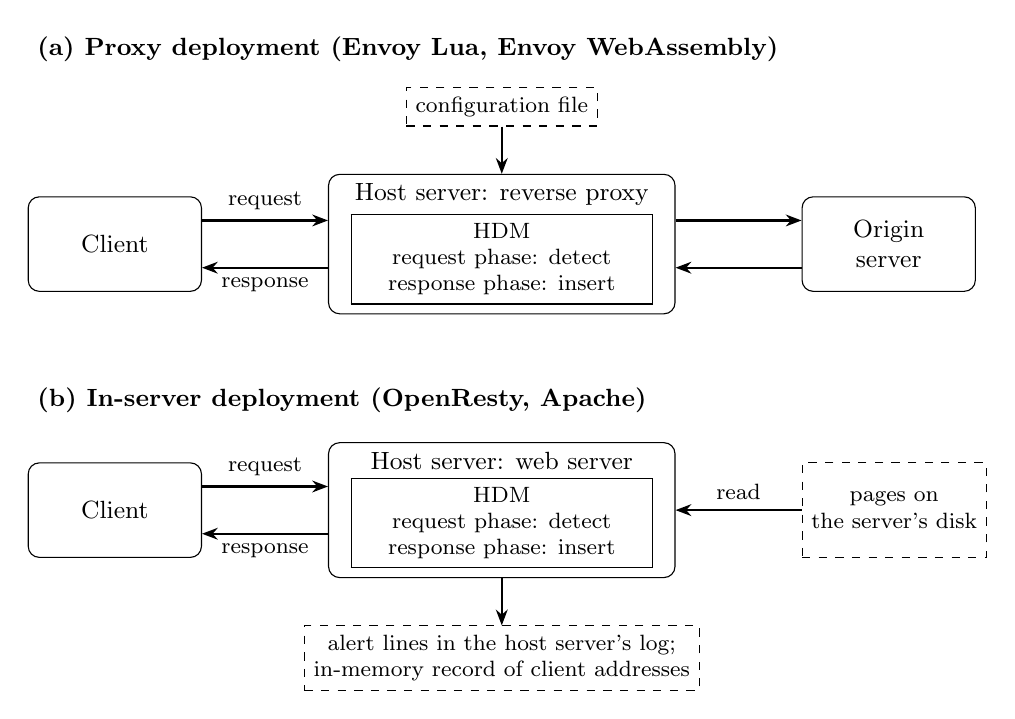
\begin{tikzpicture}[
    box/.style={draw, rounded corners, align=center, minimum height=1.2cm, font=\small},
    note/.style={draw, dashed, align=center, font=\footnotesize},
    panel/.style={font=\small\bfseries, anchor=west},
    flow/.style={-{Stealth[length=2mm]}, thick}]
  % (a) proxy deployment
  \node[box, minimum width=2.2cm] (client) {Client};
  \node[box, minimum width=4.4cm, right=1.6cm of client] (proxy)
    {Host server: reverse proxy\\[2pt]\fbox{\begin{minipage}{3.6cm}\centering\footnotesize
      HDM\\request phase: detect\\response phase: insert\end{minipage}}};
  \node[box, minimum width=2.2cm, right=1.6cm of proxy] (origin) {Origin\\server};
  \draw[flow] ([yshift=3mm]client.east) -- node[above, font=\footnotesize] {request} ([yshift=3mm]proxy.west);
  \draw[flow] ([yshift=-3mm]proxy.west) -- node[below, font=\footnotesize] {response} ([yshift=-3mm]client.east);
  \draw[flow] ([yshift=3mm]proxy.east) -- ([yshift=3mm]origin.west);
  \draw[flow] ([yshift=-3mm]origin.west) -- ([yshift=-3mm]proxy.east);
  % (b) in-server deployment
  \node[panel, below=1.1cm of client.south west, anchor=north west] (pb) {(b) In-server deployment (OpenResty, Apache)};
  \node[box, minimum width=2.2cm, below=0.5cm of pb.south west, anchor=north west] (client2) {Client};
  \node[box, minimum width=4.4cm, right=1.6cm of client2] (server)
    {Host server: web server\\[2pt]\fbox{\begin{minipage}{3.6cm}\centering\footnotesize
      HDM\\request phase: detect\\response phase: insert\end{minipage}}};
  \node[note, minimum width=2.2cm, minimum height=1.2cm, right=1.6cm of server] (disk)
    {pages on\\the server's disk};
  \draw[flow] ([yshift=3mm]client2.east) -- node[above, font=\footnotesize] {request} ([yshift=3mm]server.west);
  \draw[flow] ([yshift=-3mm]server.west) -- node[below, font=\footnotesize] {response} ([yshift=-3mm]client2.east);
  \draw[flow] (disk.west) -- node[above, font=\footnotesize] {read} (server.east);
  % shared inputs and outputs
  \node[note, below=0.6cm of server] (out) {alert lines in the host server's log;\\
    in-memory record of client addresses};
  \node[note, above=0.6cm of proxy] (config) {configuration file};
  % The heading of (a) sits above the configuration file so that its arrow does not cross it.
  \node[panel, anchor=south west, yshift=2mm] (pa) at (client.west |- config.north)
    {(a) Proxy deployment (Envoy Lua, Envoy WebAssembly)};
  \draw[flow] (config) -- (proxy);
  \draw[flow] (server) -- (out);
\end{tikzpicture}
\caption{HDM in its host server in the two deployments, which differ only in where the response comes from.}
\label{fig:design.arch}
\end{figure}

HDM has two outputs in both deployments. It writes an alert line to the log of the host server for every triggered
honeytoken, and it records the address of the client in memory. These lines are what RQ3 (functional correctness) counts when it checks whether every expected alert was raised.

%----------------------------------------------------------------------
\section{Honeytoken Types}
\label{sec:design.types}

HDM plants the five types of honeytoken listed in Table~\ref{tab:design.types}. Each is detected
through one of the three signals introduced in \secref{sec:bg.honeytokens}.

\begin{table}[htbp]
\centering
\small
\begin{tabularx}{\textwidth}{@{}l*{3}{>{\raggedright\arraybackslash}X}@{}}
\toprule
Type & Planted as & Detected when & Signal \\
\midrule
HTML comment & a comment before \texttt{</body>}, or at the end of the body if there is none
  & its trigger keyword appears in the query string & use of collected data \\
HTTP header & a decoy response header
  & its trigger keyword, the header's value, appears in the path, \texttt{Host} header or query
    string of a later request
  & data use \\
Cookie & a \texttt{Set-Cookie} header with a fixed value
  & the cookie comes back with a different value & alteration \\
Decoy path & a hidden link before \texttt{</body>}, pointing to a path the application does not use
  & a request for that path or, if so configured, for a path below it & resource request \\
Form field & a hidden input field before \texttt{</form>}
  & the field is submitted with a different value & alteration \\
\bottomrule
\end{tabularx}
\caption{The five honeytoken types of HDM and the signal by which each is detected.}
\label{tab:design.types}
\end{table}

Each honeytoken applies either to every path or to a list of exact paths, as set in the
configuration. Headers and cookies are added to every response for a matching path, whatever its
content type. Comments, links and form fields are inserted only into responses whose content type
is HTML. HDM does not check the status code or the content coding of a response before inserting
into it; Chapter~\ref{chap:AB.results}
shows what these rules mean for the HTTP mechanisms of \secref{sec:bg.http}.

Each honeytoken is defined by one entry in the configuration file (R4), in a list per type under the
key \texttt{honeytokens}. Every entry has a switch \texttt{enabled}. Every entry except the decoy
path names the paths it applies to in \texttt{paths}; the decoy path instead names the paths on
which its link is advertised. An empty \texttt{trigger\_keyword} means that the honeytoken is
detected only through the signal of Table~\ref{tab:design.types}, not through the reuse of a
value. Listings~\ref{lst:design.comment} to~\ref{lst:design.form} show one entry of each type from
the configuration used in all experiments, which contains three HTML-comment honeytokens and one
honeytoken of each other type.

\begin{lstlisting}[caption={An HTML-comment honeytoken. \texttt{comment\_value} is inserted before
\texttt{</body>} on every page; \texttt{trigger\_keyword} is searched for in the query string.},
label=lst:design.comment, float=htbp]
{
  "enabled": 1,
  "paths": ["/*"],
  "comment_value": "<!-- DEV-PORTAL: internal-admin.example.com -->",
  "trigger_keyword": "internal-admin.example.com"
}
\end{lstlisting}

\begin{lstlisting}[caption={An HTTP-header honeytoken. The header is set on every response; its
value is the trigger keyword.}, label=lst:design.header, float=htbp]
{
  "enabled": 1,
  "paths": ["/*"],
  "header_name": "X-Backend-Server",
  "header_value": "app-07.internal.example.com",
  "trigger_keyword": "app-07.internal.example.com"
}
\end{lstlisting}

\begin{lstlisting}[caption={A cookie honeytoken. HDM sets \texttt{admin\_ui=0} with the given
attributes and raises an alert when the cookie comes back with another value.},
label=lst:design.cookie, float=htbp]
{
  "enabled": 1,
  "paths": ["/*"],
  "cookie_name": "admin_ui",
  "cookie_value": "0",
  "attributes": "Path=/; SameSite=Lax",
  "trigger_keyword": ""
}
\end{lstlisting}

\begin{lstlisting}[caption={A decoy-path honeytoken. A hidden link to \texttt{trap\_path} is
inserted on every page; with \texttt{match\_type} \texttt{prefix}, a request for any path below it
also raises an alert.}, label=lst:design.decoy, float=htbp]
{
  "enabled": 1,
  "trap_path": "/api/v1/debug",
  "match_type": "prefix",
  "advertise_via": "link",
  "advertise_on_paths": ["/*"],
  "link_text": "debug console"
}
\end{lstlisting}

\begin{lstlisting}[caption={A form-field honeytoken. The hidden field \texttt{is\_admin=0} is
inserted before \texttt{</form>} on the two pages with a form; submitting it with another value
raises an alert.}, label=lst:design.form, float=htbp]
{
  "enabled": 1,
  "paths": ["/login.html", "/admin.html"],
  "field_name": "is_admin",
  "field_value": "0",
  "trigger_keyword": ""
}
\end{lstlisting}

The detectors examine the request line and headers. HDM can also inspect the bodies of form
submissions, but this option is disabled in all experiments of this thesis and is implemented in
only two of the four variants: OpenResty in-server and Envoy Lua.

%----------------------------------------------------------------------
\section{The Fake SQL-Injection Trap}
\label{sec:design.trap}

In addition to the honeytokens, HDM contains a fake login endpoint that imitates an application
vulnerable to SQL injection. The endpoint, \texttt{POST /api/login}, does not exist in the
application, in any of the variants; it exists only in HDM, and the host server answers it itself.
Requests with other methods to the same path are forwarded or served as usual, and because the
application has no such page, they are answered with status 404, the code for a resource that does
not exist (\secrefp{sec:bg.web}). Without HDM, a \texttt{POST} request to the endpoint receives
the same 404.

The SQL-injection trap reads the watched form fields of the request body, \texttt{username} and then
\texttt{password}. It decodes each value, converts it to lower case and collapses whitespace, and
then searches it for a list of 22 literal signatures, such as \texttt{' or}, \texttt{union select}
and \texttt{sleep(}, which correspond to the probes described in \secrefp{sec:bg.sqli}. The
signatures are matched as plain substrings rather than as regular expressions, which are not
available alike in all variants.
\begin{itemize}
  \item \emph{Signature found.} HDM writes an alert, records the client address and returns
    status 500 with a page that imitates a MySQL syntax error. The page reflects the attacker's
    input, HTML-escaped and truncated to 200 characters, inside a plausible \texttt{SELECT}
    statement.
  \item \emph{No signature found.} HDM writes an \emph{SQL-injection trap line}, a log line that records the
    attempt without raising an alert, and returns status 401 with a ``sign in failed'' page, so that
    the endpoint behaves like a real login. 
\end{itemize}

%----------------------------------------------------------------------
\section{Per-Request Processing}
\label{sec:design.pipeline}

Everything that depends only on the configuration is computed once, when the configuration is
loaded: for every configured path, HDM prepares a plan that holds the comments, headers, cookies
and markup to insert into responses for that path. For each request, HDM then performs the
following steps, which Figure~\ref{fig:design.flow} summarises.

\begin{figure}[htbp]
\centering
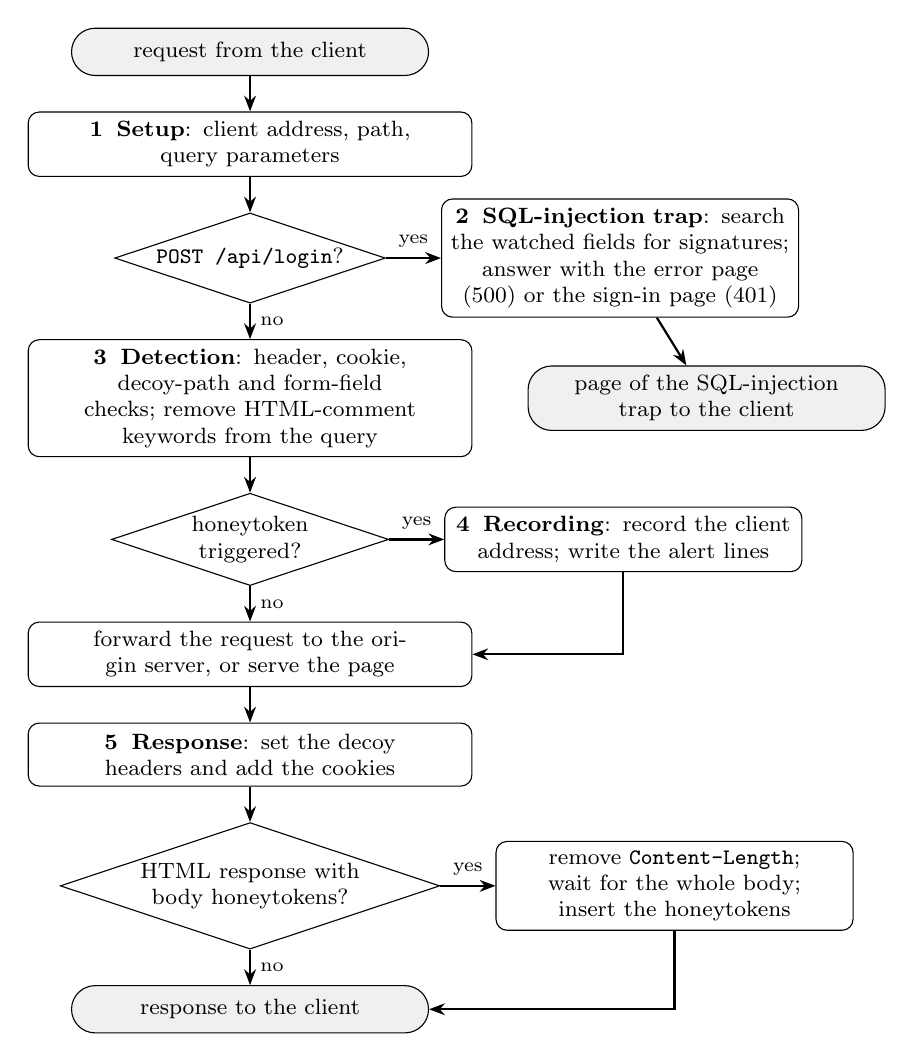
\begin{tikzpicture}[
    node distance=4.5mm and 7mm,
    stage/.style={draw, rounded corners, align=center, font=\footnotesize, text width=5.4cm,
      minimum height=8mm},
    side/.style={draw, rounded corners, align=center, font=\footnotesize, text width=4.3cm,
      minimum height=8mm},
    decision/.style={draw, diamond, aspect=3, align=center, font=\footnotesize, inner sep=1pt},
    term/.style={draw, rounded corners=3mm, align=center, font=\footnotesize, fill=gray!12,
      minimum height=6mm, text width=4.3cm},
    flow/.style={-{Stealth[length=2mm]}, thick},
    lbl/.style={font=\scriptsize}]
  \node[term] (in) {request from the client};
  \node[stage, below=of in] (setup) {\textbf{1\enspace Setup}: client address, path,\\ query parameters};
  \node[decision, below=of setup] (trapq) {\texttt{POST /api/login}?};
  \node[side, right=of trapq] (trap) {\textbf{2\enspace SQL-injection trap}: search the watched fields for
    signatures; answer with the error page (500) or the sign-in page (401)};
  \node[stage, below=of trapq] (detect) {\textbf{3\enspace Detection}: header, cookie, decoy-path
    and form-field checks; remove HTML-comment keywords from the query};
  \node[term, right=of detect] (trapout) {page of the SQL-injection trap to the client};
  \node[decision, below=of detect] (hitq) {honeytoken\\triggered?};
  \node[side, right=of hitq] (record) {\textbf{4\enspace Recording}: record the client address;
    write the alert lines};
  \node[stage, below=of hitq] (fwd) {forward the request to the origin server, or serve the page};
  \node[stage, below=of fwd] (resp) {\textbf{5\enspace Response}: set the decoy headers and add the
    cookies};
  \node[decision, below=of resp] (htmlq) {HTML response with\\body honeytokens?};
  \node[side, right=of htmlq] (insert) {remove \texttt{Content-Length}; wait for the whole body;
    insert the honeytokens};
  \node[term, below=of htmlq] (out) {response to the client};
  \draw[flow] (in) -- (setup);
  \draw[flow] (setup) -- (trapq);
  \draw[flow] (trapq) -- node[lbl, above] {yes} (trap);
  \draw[flow] (trap) -- (trapout);
  \draw[flow] (trapq) -- node[lbl, right] {no} (detect);
  \draw[flow] (detect) -- (hitq);
  \draw[flow] (hitq) -- node[lbl, above] {yes} (record);
  \draw[flow] (record.south) |- (fwd.east);
  \draw[flow] (hitq) -- node[lbl, right] {no} (fwd);
  \draw[flow] (fwd) -- (resp);
  \draw[flow] (resp) -- (htmlq);
  \draw[flow] (htmlq) -- node[lbl, above] {yes} (insert);
  \draw[flow] (insert.south) |- (out.east);
  \draw[flow] (htmlq) -- node[lbl, right] {no} (out);
\end{tikzpicture}
\caption{Per-request processing of HDM: steps 1 to 4 run in the request phase and step 5 in the response phase.}
\label{fig:design.flow}
\end{figure}
\begin{enumerate}
  \item \emph{Setup.} The client address is taken from the network connection, not from a header
    that the client could set. The path is the request target up to the first \texttt{?}, used
    without decoding. The query string is split once into its parameters, in their original order;
    a parameter is decoded only if it contains an encoded character.
  \item \emph{SQL-injection trap.} A \texttt{POST} request to \texttt{/api/login} is handed to the SQL-injection trap
    (\secrefp{sec:design.trap}), and processing ends there.
  \item \emph{Detection.} The detectors for headers, cookies, decoy paths and form fields run in a
    fixed order. HDM then searches the decoded query parameters for the trigger keywords of the HTML
    comments. A parameter that contains a keyword is removed, and the query string is rebuilt from
    the original text of the remaining parameters, so that their order and encoding are kept (R2).
  \item \emph{Recording.} If any honeytoken was triggered, HDM records the client address and
    writes one alert line per triggered honeytoken, with line breaks in attacker-controlled
    values replaced (R3).
  \item \emph{Response.} HDM looks up the plan for the path, sets the decoy headers and adds the
    cookies. If the response is HTML and the plan inserts into the body, HDM removes the
    \texttt{Content-Length} header, because the length of the body changes
    (\secrefp{sec:bg.http}), waits until the whole body has arrived
    (\secrefp{sec:bg.proxy}), and inserts each honeytoken at its anchor, found by a plain,
    case-sensitive search.
\end{enumerate}

These steps are the specification that every variant implements, in either deployment.
Chapter~\ref{chap:impl} describes how each of the four variants realises them and how it was
verified that the variants behave identically (R5).

%======================================================================
\chapter{Implementation of the Variants}
\label{chap:impl}

Chapter~\ref{chap:design} specified HDM independently of any host server. This chapter describes
how the four variants implement that specification and how they were made comparable.
\secref{sec:impl.common} gives the structure that all of them share,
Sections~\ref{sec:impl.openresty}--\ref{sec:impl.apache} describe only what is particular to each
variant, \secref{sec:AB.level} describes how the variants were levelled, and
\secref{sec:impl.parity} describes the check that they behave identically.

%----------------------------------------------------------------------
\section{Common Structure}
\label{sec:impl.common}

All four variants read the same configuration file (R4) and implement the five steps of
\secref{sec:design.pipeline} in the same order. In OpenResty and Apache httpd, HDM is Lua code
run by the server's Lua module; in Envoy, it is an HTTP filter (\secrefp{sec:bg.platforms}).
Each variant compiles the configuration into its per-path plans when it loads it, checks the request
in the hook that the host server runs before the request is forwarded or served, and inserts the
honeytokens in the hooks that see the response (\secrefp{sec:bg.platforms}): steps 1 to 4 run
in the request phase and step 5 in the response phase.

In the in-server variants, the removal of trigger keywords (step~3 of
\secref{sec:design.pipeline}) is still performed, but nothing reads the cleaned query once the
page has been chosen. There, R2 holds trivially, and the detection can be checked only through the
alert lines (\secrefp{sec:impl.parity}).

Every variant also contains timers around its detection and insertion steps. When the
configuration enables them, each timer writes a \emph{timing line} to the log of the host server: a
log line that records how long one operation took, in microseconds. The timing lines show what
HDM's own operations cost, which the latency and the CPU time of a request cannot separate from the
work of the host server. Because writing them costs time as well, they are switched on in only one
of the configurations that Chapter~\ref{chap:method} measures (\secrefp{sec:method.tiers}).

%----------------------------------------------------------------------
\section{OpenResty (In-Server) }
\label{sec:impl.openresty}

In OpenResty in-server, nginx serves the pages itself from a directory on disk, its root directory
\cite{nginx_core}, and HDM is Lua code that the \texttt{lua-nginx-module} runs. HDM's hooks are set once for the whole server, so that every location of the
server inherits them. HDM compiles the configuration once, before nginx starts its worker
processes, so that every worker inherits the compiled plans. The client addresses that HDM records
are kept in a shared memory zone that all worker processes use \cite{luanginx}. Because nginx passes
the response body to the extension in pieces (\secrefp{sec:bg.platforms}), the body filter
collects the pieces and inserts the honeytokens when the last one has arrived.

One detail of serving the pages affects HDM directly. A request for \texttt{/} names a directory,
not a page. nginx resolves such a request by an internal redirect to the index page
\cite{nginx_index}, and the redirected request passes through
the access phase, and with it through HDM's detection, a second time, so that one request for
\texttt{/} that carries a trigger keyword would raise two alerts. OpenResty in-server therefore maps \texttt{/} directly to the index page, with a mapping that
serves the file it finds in the current context, without a redirect \cite{nginx_core}; with this mapping, such a request raises one alert.

OpenResty in-server is the reference variant, against which the others are compared in
\secref{sec:impl.parity}.

%----------------------------------------------------------------------
\section{Envoy with a Lua Filter}
\label{sec:impl.envoylua}

This variant runs HDM as an Envoy HTTP filter written in Lua, in a reverse proxy in front of the
origin server. Each worker thread loads and compiles the configuration in its own Lua state. In the
response phase, the filter waits until Envoy has buffered the whole body, within Envoy's buffer
limits (\secrefp{sec:bg.platforms}), and writes the modified body back. Because Envoy then
knows the final length, it sends a \texttt{Content-Length} header with an injected page, as Apache
in-server was also measured to do; OpenResty in-server and the WebAssembly variant send an injected
page without one, in chunks (\secrefp{sec:bg.http}). 

Requests to the fake login endpoint of the
SQL-injection trap (\secrefp{sec:design.trap}) are answered by the filter itself and never reach the
origin server; the WebAssembly variant cannot do this (\secrefp{sec:impl.wasm}).

%----------------------------------------------------------------------
\section{Envoy with a WebAssembly Filter}
\label{sec:impl.wasm}

This variant implements HDM in Rust against the Proxy-Wasm interface and compiles it to a
WebAssembly module, the binary file of compiled code that Envoy's WebAssembly filter loads
(\secrefp{sec:bg.platforms}); Envoy runs it on the V8 engine (\secrefp{sec:bg.runtimes}).

The module and Envoy communicate in two directions, as Figure~\ref{fig:impl.wasm} shows. Envoy calls
functions of the module at fixed steps of each exchange: when the request headers have arrived, for
each piece of the request body, when the response headers have arrived, and for each piece of the
response body. The module, in turn, can reach the request and the response only by calling
functions that Envoy provides, for example to read a header, to read or replace a body, to answer a
request itself, or to write a log line; the values these functions return are written into the
module's own memory \cite{proxywasm_spec,haas2017wasm}.

\begin{figure}[htbp]
\centering
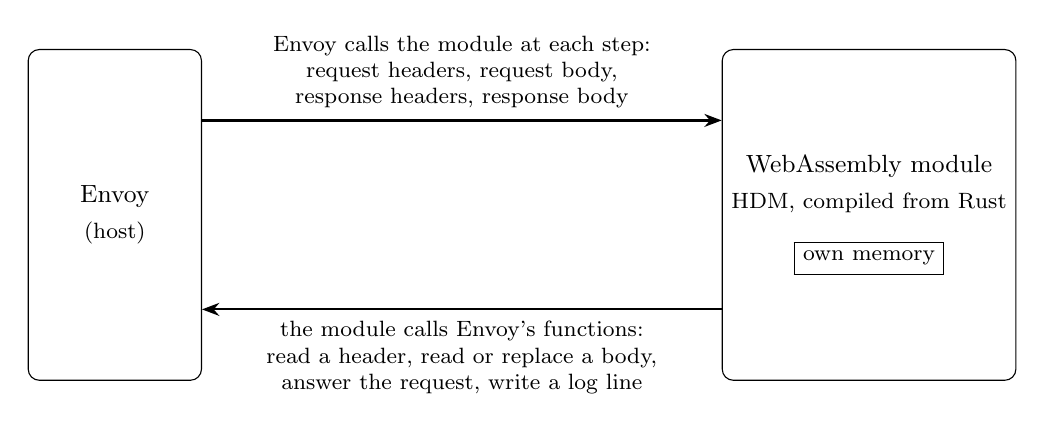
\begin{tikzpicture}[
    box/.style={draw, rounded corners, align=center, font=\small, minimum height=4.2cm},
    lbl/.style={font=\footnotesize, align=center, inner sep=3pt},
    flow/.style={-{Stealth[length=2.2mm]}, thick}]
  \node[box, minimum width=2.2cm] (envoy) {Envoy\\[2pt]\footnotesize(host)};
  \node[box, minimum width=3.3cm, right=6.6cm of envoy] (mod)
    {WebAssembly module\\[2pt]\footnotesize HDM, compiled from Rust\\[8pt]
     \fbox{\footnotesize own memory}};
  \draw[flow] ([yshift=12mm]envoy.east) -- node[lbl, above=1pt] {Envoy calls the module at each step:\\
    request headers, request body,\\response headers, response body} ([yshift=12mm]mod.west);
  \draw[flow] ([yshift=-12mm]mod.west) -- node[lbl, below=1pt] {the module calls Envoy's functions:\\
    read a header, read or replace a body,\\answer the request, write a log line} ([yshift=-12mm]envoy.east);
\end{tikzpicture}
\caption{How Envoy and the WebAssembly module of the WebAssembly variant communicate.}
\label{fig:impl.wasm}
\end{figure}

Because every read of a request header is such a call from the module into Envoy, the module asks
for each header at most once and only when it needs it. It reads the request method only for
requests to \texttt{/api/login}, the path of the SQL-injection trap, and it reads the
\texttt{Cookie} header only when the configuration contains a cookie honeytoken. Envoy passes the
configuration file to the module at start-up, and the module compiles it once. In the response
phase, the module lets the headers continue before the body arrives, removing their
\texttt{Content-Length} when the page will
be injected, and then waits for the whole body and inserts the honeytokens into its bytes.

The SQL-injection trap cannot be implemented here as in the other variants. As Figure~\ref{fig:impl.wasm} shows, Envoy
hands a request to the module in separate steps: first when the request headers have arrived, and again when the
request body has arrived. In the Envoy release used in this thesis, 1.30
(\secrefp{sec:method.testbed}), the module can answer a request itself only in the first step.
The SQL-injection trap, however, needs the request body, which is only available in the second
step: an answer given there is rejected, and holding the request back in the first step until the
body arrives stops the request altogether. This variant therefore lets the
request continue to the origin server. The origin server has no \texttt{/api/login}, because the
endpoint exists only in HDM (\secrefp{sec:design.trap}), and answers with status 404. Meanwhile,
the module examines the request body when it arrives, and in the response phase it replaces the
origin server's 404 with the page of the SQL-injection trap. The client receives the same response as from the other variants
(\secrefp{sec:impl.parity}), at the cost of one additional round trip to the origin server.

%----------------------------------------------------------------------
\section{Apache httpd In-Server}
\label{sec:impl.apache}

In Apache in-server, Apache httpd serves the pages itself from a directory on disk \cite{apache_request}. HDM consists of three Lua scripts that Apache httpd's Lua module runs
(\secrefp{sec:bg.platforms}): one for the request phase, one for the SQL-injection trap and one
for the response body. The three share a common Lua library that reads and compiles the
configuration.

The script for the request phase runs in the step in which Apache checks
whether access to the resource is allowed (\secrefp{sec:bg.platforms}). It performs steps 1, 3
and 4 of \secref{sec:design.pipeline}: it looks up the plan for the path, searches the request
for trigger keywords and records the alerts. It also prepares the decoy header and the cookie
honeytoken already in this phase, in the set of response headers that Apache sends with error
responses as well, so that they reach the client whether the requested page exists or not. The script for the response body is an output filter. It collects the body piece by piece and
inserts the honeytokens when the last piece has arrived. Because the insertion changes the length
of the body, the Apache configuration removes the \texttt{Content-Length} header from every
response (\secrefp{sec:bg.http}). Apache httpd renders its own error pages, such as
the page for a missing resource (status 404). No honeytoken is therefore inserted into Apache's own error pages; the decoy header and
cookie, prepared in the request phase, are still sent.

A separate handler script is registered for the path
\texttt{/api/login}. For a \texttt{POST} request, it reads the request body, scans it for the attack
signatures and writes the answer itself (\secrefp{sec:design.trap}): status 500 with the fake
database error if a signature matches, and status 401 otherwise. The request therefore never
reaches Apache's serving of files. The script for the request phase leaves these requests to the
response handler, so they raise no alert for a trigger keyword and carry no decoy header, as in the other
variants. For any other method, the response handler passes the request on, and Apache answers with status
404, because no such page exists.

%----------------------------------------------------------------------
\section{Levelling the Variants}
\label{sec:AB.level}

R5 requires that the variants behave identically, and a fair comparison requires that no variant
pays for work that the others do not do. The variants are therefore aligned in four respects.

\paragraph{Behaviour.} All four variants implement the procedure of
\secref{sec:design.pipeline} step by step: they parse the query in the same way, search it for
the trigger keywords literally, so that characters such as \texttt{-} and \texttt{.} in a keyword
have no special meaning, rebuild it in the same way, take the client address from the connection
and write the same alert lines. \secref{sec:impl.parity} checks that they do.

\paragraph{Defaults of the server software.} Where the server software differs in a default that affects cost, the default
is aligned. OpenResty and Apache httpd write an access-log line for every request by default, which
Envoy does not, so these logs are switched off; for the Envoy variants, the origin server's log
still records every forwarded request. Apache by default checks every script for changes each time
it runs it, while the other variants load their code once, so Apache is configured to load its
scripts once. All variants run on the public container images of the server software, so every other
default is its own.

\paragraph{Test responses.} RQ3 (functional correctness) is checked with a set of requests whose
responses the main workload does not contain (\secrefp{sec:method.supp}). Each variant's
response with HDM is compared with its own response without HDM and marked as preserved, injected,
changed or broken. Two of these requests ask for responses that no page on disk provides: a page
compressed with gzip and an empty response with status 204. In the Envoy variants, these requests are
forwarded, and the origin server produces both responses through its own configuration: it
compresses the pages of one directory, and it answers one path with an empty 204 response. The
in-server variants have no origin server. Without further configuration, they would send the page
uncompressed and answer the second path with status 404, because no such file exists, so they
would not be tested on these two kinds of response at all. Each in-server variant is therefore
configured to produce both responses itself, as the origin server does, and all four variants are
checked on the same cases.


\paragraph{Configurations without HDM.} Each variant's configuration without HDM, which
Chapter~\ref{chap:method} uses as the baseline, was derived from its configuration with HDM by
deleting the HDM parts and nothing else, and it runs in the same container. For the in-server
variants, the result is the web server serving its own pages, with the mappings of
Sections~\ref{sec:impl.openresty} (\emph{\nameref{sec:impl.openresty}}) and~\ref{sec:impl.apache} (\emph{\nameref{sec:impl.apache}}) and the test responses unchanged. Two
differences are kept on purpose, because they are part of what HDM costs: injected responses are
larger, and OpenResty in-server and the WebAssembly variant send them in chunks, without a
\texttt{Content-Length} header.

%----------------------------------------------------------------------
\section{Verifying Equivalence}
\label{sec:impl.parity}

R5 (\secrefp{sec:design.req}) requires that, for the same request, every variant returns the same
response, writes the same alerts and forwards, or serves, the same request. The levelling of
\secref{sec:AB.level} aligns the variants by construction. This section describes how it was
checked that they also behave identically in practice, and which differences remain.

Such a check is needed because the variants are four separate implementations: three in Lua, each
written against the interface of a different host server, and one in Rust. Each also depends on how
its host server parses a request and passes it on. Differences can therefore hide in details that
the benchmark requests do not exercise, such as encoded keywords, the order of the parameters that
remain after a keyword is removed, or form fields that occur twice. At the same time, the responses
of the variants cannot simply be compared byte for byte. Some parts of a response, such as the body
of an error page, are produced by the server and not by HDM, and the in-server variants have no
origin server to which they could forward a request.

The variants are therefore compared by an automated parity check. It sends the same 13 requests to
every variant: the four \texttt{GET} requests of the benchmark (Chapter~\ref{chap:method}) and nine
further cases, among them encoded keywords, the order of the remaining parameters after a keyword is
removed, duplicated form fields, a path below the decoy path, and a signature hit and a clean login
at the SQL-injection trap (Appendix~\ref{app:parity}). For each request, it records what the client
receives (status, decoy header, cookies and a hash of the body), the alert lines the variant writes,
and the requests that reach the origin server, as recorded in the origin's log.

Each variant is compared with a reference, OpenResty in-server, by four rules that separate what
HDM does from what the server does:
\begin{enumerate}
  \item Status, decoy header and cookies must match the reference for every request.
  \item The hash of the body must match wherever the reference returned a page with status 200.
    Error pages are rendered by whichever server produced them and differ by construction.
  \item The alert lines must be identical.
  \item Because the reference sends nothing to the origin server, the requests that reach it are
    checked on their own terms: the in-server variants must send none, and the two Envoy variants
    must forward the same requests.
\end{enumerate}

\begin{table}[!ht]
\centering
\small
\begin{tabularx}{\textwidth}{@{}>{\raggedright\arraybackslash}p{4.6cm}>{\raggedright\arraybackslash}p{2.6cm}X@{}}
\toprule
Difference & Variant & Reason \\
\midrule
Framing of injected responses & OpenResty in-server and Envoy WebAssembly against the others
  & These send injected pages in chunks; Envoy Lua and Apache in-server send a
  \texttt{Content-Length} that matches the injected body (\secrefp{sec:impl.envoylua}) \\ \addlinespace
At most one cookie honeytoken per path & Apache in-server & Apache httpd's Lua module can only replace a
  \texttt{Set-Cookie} header, not add a second (\secrefp{sec:impl.apache}); the configuration
  plants one \\ \addlinespace
Requests to the SQL-injection trap reach the origin server & Envoy WebAssembly & A constraint of the module
  interface (\secrefp{sec:impl.wasm}); the client's response is identical \\ \addlinespace
Body of error pages, such as status 404 & all & Rendered by the host server itself in the
  in-server variants and by the origin server in the Envoy variants; status, decoy header and
  cookie are identical \\ \addlinespace
No honeytokens inserted into the server's own error pages & Apache in-server & Apache removes
  resource-level output filters before it renders an error page (\secrefp{sec:impl.apache});
  the decoy header and cookie are still sent \\ \addlinespace
No request reaches the origin server & Both in-server variants & There is no origin server in the
  request path; the removal of keywords is checked through the alert lines only \\ \addlinespace
No decoy header on the 204 test response & Apache in-server & The response is produced before the
  access checks run (\secrefp{sec:AB.level}); no benchmark request asks for it \\
\bottomrule
\end{tabularx}
\caption{Differences between the variants that remain after levelling.}
\label{tab:impl.residuals}
\end{table}

The check leaves the differences listed in Table~\ref{tab:impl.residuals}, which are excluded from
the comparison. None of them changes the body of a page with status 200 that a client receives, or the
alerts a variant writes. Run on the code that produced the results of
Chapter~\ref{chap:AB.results}, the check found no other difference from the reference. For the 13
requests, every variant wrote the same 11 alert lines and one SQL-injection trap line. Both Envoy variants
forwarded the same 11 requests to the origin server, none of them carrying a trigger keyword, and
the WebAssembly variant's requests to the SQL-injection trap in addition; the in-server variants sent none.

%======================================================================
\chapter{Evaluation Methodology}
\label{chap:method}

Chapter~\ref{chap:impl} made the four variants do the same work. This chapter describes how the
cost of that work was measured. The effect to be measured is small: the operations of HDM take
microseconds, and a request takes less than a millisecond without HDM, on a virtualised host whose
timing drifts by hundreds of microseconds. A difference between two separate runs would therefore
reflect the drift as much as HDM, and the method is built around one principle: every cost is a
difference between two configurations measured minutes apart in the same run, never a difference
between separate runs. Sections~\ref{sec:AB.metrics} to~\ref{sec:method.planes} describe the
experiments, the testbed, the workload, the configurations compared and what is measured.
\secref{sec:method.supp} describes the supplementary experiments,
\secref{sec:AB.validity} the rules by which a run is accepted or rejected, and
what the method cannot resolve.

%----------------------------------------------------------------------
\section{Experiments and Metrics}
\label{sec:AB.metrics}

The research questions are answered by one main experiment and two
supplementary ones, listed in Table~\ref{tab:method.rq}. The main experiment, the \emph{paired
benchmark}, is named after this principle: within one run, it measures every variant with and
without HDM and pairs the two (\secrefp{sec:method.tiers}). It measures latency, CPU time, the duration of HDM's operations and the integrity of
responses under load for all four variants. The supplementary experiments each answer one question
that the main workload cannot: the \emph{functional matrix} checks how HDM treats other kinds of
response, and the \emph{request-type and page-size runs} measure how the cost divides between
request types and grows with the size of a page (\secrefp{sec:method.supp}).

\begin{table}[!t]
\centering
\small
\begin{tabularx}{\textwidth}{@{}>{\raggedright\arraybackslash}p{3.6cm}>{\raggedright\arraybackslash}p{2.9cm}>{\raggedright\arraybackslash}X@{}}
\toprule
Question & Experiment & Metric \\
\midrule
RQ1 (latency added, against a reverse proxy's own, as load grows) & paired benchmark & latency added per \texttt{GET} request at the median and the 95th
  percentile; latency of the reverse proxy without and with HDM above the origin server \\ \addlinespace
RQ2.1 (CPU time added per request) & paired benchmark & CPU time added per request \\ \addlinespace
RQ2.2 (where the added cost arises) & paired benchmark; request-type and page-size runs & share of the added CPU time inside
  HDM's timed code; CPU time of the \texttt{GET} requests against those to the SQL-injection trap; latency against page
  size \\ \addlinespace
RQ3.1 (the same response with and without HDM) & functional matrix & response with HDM against the response without it, per kind of
  response \\ \addlinespace
RQ3.2 (responses intact under load) & paired benchmark & share of responses identical to the reference response \\ \addlinespace
RQ3.3 (every expected alert raised) & paired benchmark & alert lines and SQL-injection trap lines written, against those expected \\ \addlinespace
RQ4.1 (cost per honeytoken type in each runtime) & paired benchmark & duration of HDM's operations per honeytoken type \\ \addlinespace
RQ4.2 (cost of decoding and scanning in the SQL-injection trap) & paired benchmark & duration of the SQL-injection trap's work for each of its four probes \\ \addlinespace
RQ4.3 (reverse proxy against web server on the same runtime) & paired benchmark; functional matrix & the metrics of RQ1 (latency), RQ2.1 (CPU time) and RQ3.1 (responses with and without HDM) for Envoy Lua
  and OpenResty in-server side by side \\
\bottomrule
\end{tabularx}
\caption{The experiments and metrics that answer each research question.}
\label{tab:method.rq}
\end{table}

The four variants are arranged so that RQ4 can separate the effects of the runtime, the host server
and the deployment. The two Envoy
variants share a host server and a deployment but differ in runtime. Envoy Lua and OpenResty
in-server share LuaJIT but differ in host server and deployment, which is the comparison of RQ4.3.
The two in-server variants share a deployment but differ in both host server and runtime: Apache
is the only variant whose extension code is always interpreted, and because it differs
from OpenResty in the server as well, a difference between the two cannot be attributed
to the runtime alone.

%----------------------------------------------------------------------
\section{Testbed}
\label{sec:method.testbed}

All measurements were taken on one virtual machine (VM) under VirtualBox, with eight virtual CPUs
(vCPUs) and 7.8\,GiB of memory, on a laptop with an Intel Core i7-13650HX processor. The guest runs
Kali Linux with Linux kernel~6.12 and Docker~27.5. Every component runs in its own container
(\secrefp{sec:bg.perf}), and all containers share one Docker bridge network:
\begin{itemize}
  \item the load generator, k6~2.0, which sends the requests and records their latency;
  \item the origin server, nginx~1.29 in the \texttt{nginx:alpine} image, which serves five static
    HTML pages of 864 to 1,396~bytes and the generated test pages of the supplementary experiments;
  \item the host server of the variant under test: OpenResty~1.27.1, Envoy~1.30.11 or Apache
    httpd~2.4.67, whose Lua module uses PUC Lua~5.1.5.
\end{itemize}
The images are referenced by tags that can move, such as \texttt{latest}, and their identifiers
were recorded for the run of the in-server variants only.

Three measures keep the components from disturbing one another. First, each container is pinned to
its own vCPUs: the host server to two (vCPUs~1 and~2), the origin server to one (vCPU~3) and the
load generator to four (vCPUs~4 to~7), with vCPU~0 left to the operating system. Without this, the
load generator's own scheduling delay would be part of every latency it records. Second, the
containers deliver their log lines without blocking and with a buffer of 64\,MB. With
\emph{blocking} delivery, Docker's default, a process that writes a log line waits until the line
has been handed on; with \emph{non-blocking} delivery, the line is placed in a buffer and the process
continues at once, and when the buffer is full, new lines are dropped \cite{docker_logging}. With
blocking delivery, a worker whose log pipe is full stalls in the middle of a request; the instrumented
configuration writes about 39 timing lines per iteration of the workload
(\secrefp{sec:method.workload}), and a stall that falls inside a timed operation is charged to
HDM. The cost of non-blocking delivery is that a line may be lost under an
extreme burst, which would show up as a missing sample rather than as a wrong one. Third, before
every reportable run the guest was tuned: transparent huge pages and swapping were disabled.
With \emph{transparent huge pages}, the Linux kernel maps a process's memory in large pages on its
own, without being asked, and to obtain such pages it may first move other pages together; with
\emph{swapping}, it moves pages that a process has not used recently to disk and reads them back
when the process needs them again \cite{kernel_mm_concepts}. Both can stall a running process for
milliseconds, and also, periodic maintenance services were stopped.

Pinning has a side effect that differs between the servers. With the setting \texttt{auto}, nginx
sizes its pool of worker processes from the number of processors that the C library reports, and the
C library of the OpenResty image ignores the pinning: OpenResty starts eight workers on its two vCPUs.
The C library of the origin server's image, musl, respects the pinning, and the origin server starts
one worker. Apache httpd sizes its pool from fixed defaults. These worker counts were recorded in
every result file and left as they are. They are the same in the configurations with and without
HDM and therefore cancel in every cost of HDM, but they are one of the differences between the
variants when the variants are compared with one another.

The two deployments use the same core assignment, and this matters for what can be compared. In the
proxy deployment, the server-side work of a request is spread over three vCPUs, two for the reverse
proxy and one for the origin server. In the in-server deployment, all of it, including reading the
file and sending it, runs on the two vCPUs of the host server, and the origin server's vCPU is idle.
This is why the thesis compares latency and CPU time per request between the variants but not
capacity, the highest request rate a variant sustains: a comparison of capacity would compare two
vCPUs with three.

%----------------------------------------------------------------------
\section{Workload}
\label{sec:method.workload}

The load generator sends requests in \emph{iterations}. Each iteration consists of nine requests: one
unrecorded \texttt{GET /}, followed by eight \emph{probes}, each of which exercises one part of HDM
(Table~\ref{tab:method.probes}). The first request is sent but not recorded because the first
request on a connection that has been idle pays a setup cost that the following requests do not;
it absorbs that cost, so that all eight probes are measured on an equally warm connection. Without HDM, the four \texttt{POST} requests are answered with 404,
because the application has no such endpoint.

\begin{table}[htbp]
\centering
\small
\begin{tabularx}{\textwidth}{@{}>{\raggedright\arraybackslash}p{5.6cm}>{\raggedright\arraybackslash}X>{\raggedright\arraybackslash}p{2.4cm}@{}}
\toprule
Request & What HDM does & Response \\
\midrule
\texttt{GET /} & inserts the honeytokens; nothing to detect & 200 \\ \addlinespace
\texttt{GET /api/login?\allowbreak password=}\textit{keyword} & detects and removes the keyword of an HTML
  comment & 404 \\ \addlinespace
\texttt{GET /login.html?\allowbreak is\_admin=1\&\allowbreak probe=}\textit{value}, with the cookie \texttt{admin\_ui=1}
  & detects a changed form field, a replayed header value and a changed cookie, three alerts & 200 \\ \addlinespace
\texttt{GET /api/v1/debug} & detects a request for the decoy path & 404 \\ \addlinespace
\texttt{POST /api/login} with a signature, plain & SQL-injection trap: signature found & 500 \\ \addlinespace
\texttt{POST /api/login} with a signature, percent-encoded & SQL-injection trap: decodes the input, signature found & 500 \\ \addlinespace
\texttt{POST /api/login} without a signature, plain & SQL-injection trap: no signature found & 401 \\ \addlinespace
\texttt{POST /api/login} without a signature, percent-encoded & SQL-injection trap: decodes the input, no signature found & 401 \\
\bottomrule
\end{tabularx}
\caption{The eight probes of an iteration and the response of a variant with HDM.}
\label{tab:method.probes}
\end{table}

The four \texttt{GET} probes are the requests on which latency is reported. Two of them end in a 404,
because the application has neither a page \texttt{/api/login} nor the decoy path; their 404 pages
are HTML and receive honeytokens like the other pages, except in Apache in-server
(\secrefp{sec:impl.apache}). Together with the unrecorded first request,
an iteration therefore contains five HTML responses into which HDM inserts honeytokens. With HDM,
one iteration should produce seven alert lines (one for the HTML comment, three for the tampered
request, one for the decoy path and two for the signature hits) and two SQL-injection trap lines for the
clean logins. The four probes of the SQL-injection trap form a two-by-two design, whether a signature is found crossed with
whether the input must be decoded, because the two factors affect its cost in opposite
directions and a single pair of probes would confound them. Its timers, read separately for
each of the four probes, therefore separate the cost of decoding from the cost of scanning
(RQ4.2).

The eight probes are not sent in a fixed order, because some requests leave state behind that
affects the next one: Apache httpd, for example, closes the connection after the SQL-injection
trap's response with status 500, so the request that follows has to open a new one. In a fixed
order, this cost would always be charged to the same probe. The order therefore changes from
iteration to iteration according to a \emph{Williams design}, a scheme for ordering a set of
treatments, here the probes, so that each is preceded equally often by every other
\cite{williams1949designs}. Over eight consecutive iterations, every probe takes every position
once, so that no probe is always the first or the last of an iteration, and follows every other
probe exactly once. The cost that one probe leaves to the next is thereby spread over all probes.

Requests are generated according to an \emph{open} model. In a closed model, a new request is sent
only when an earlier one has completed, whereas in an open model requests arrive independently of
completions \cite{schroeder2006open}. Schroeder et al.\ show that the two models can behave very
differently \cite{schroeder2006open}. Under a closed model, the configuration that responds more
slowly also receives less load \cite{k6_openclosed}, so two configurations would not be measured under
the same load. The
benchmark therefore uses k6's constant-arrival-rate executor, which starts iterations at a fixed
rate, independently of the response times of the system under test \cite{k6_openclosed}. If k6 has
no free simulated user to start an iteration on time, it records the iteration as dropped
\cite{k6_dropped}, and \secref{sec:AB.validity} treats a shortfall of this kind as a failed
run rather than as a lower load.

The paired benchmark offers three rates: 1, 10 and 100 iterations per second, that is 9, 90 and
900 requests per second. Each measurement lasts 90, 45 or 30 seconds respectively, so that it
contains 90, 450 or 3,000 iterations. A five-second delay before the first iteration gives slowly
starting servers time to finish initialising.

%----------------------------------------------------------------------
\section{Tiers and Pairing}
\label{sec:method.tiers}

Every variant is measured in four configurations, called \emph{tiers}
(Table~\ref{tab:method.tiers}). They differ in which server answers the load generator's requests,
in whether HDM is present, and in whether HDM writes its timing lines (\secrefp{sec:impl.common}).
In the table, nginx is the plain web server that holds the pages; in the proxy deployment, it is the
origin server behind Envoy. The configuration file of the silent tier is generated from that of
the instrumented tier at the start of every run and differs from it in a single setting, which
switches the timing lines off. The configuration without HDM was derived from the configuration with
HDM by deleting the HDM parts and nothing else (\secrefp{sec:AB.level}).

\begin{table}[htbp]
\centering
\small
\begin{tabularx}{\textwidth}{@{}l>{\raggedright\arraybackslash}X>{\raggedright\arraybackslash}X ll@{}}
\toprule
 & \multicolumn{2}{l}{Requests are answered by} & & \\
\cmidrule(lr){2-3}
Tier & proxy variants & in-server variants & HDM & Timing lines \\
\midrule
origin & nginx alone & not reported & no & --- \\ \addlinespace
bare & Envoy, forwarding to nginx & OpenResty or Apache httpd & no & --- \\ \addlinespace
silent & Envoy, forwarding to nginx & OpenResty or Apache httpd & yes & off \\ \addlinespace
instrumented & Envoy, forwarding to nginx & OpenResty or Apache httpd & yes & on \\
\bottomrule
\end{tabularx}
\caption{The four tiers in which every variant is measured.}
\label{tab:method.tiers}
\end{table}

The four tiers are the following:
\begin{itemize}
  \item \emph{origin}: the load generator sends its requests directly to nginx, which serves the
    pages on its own. The variant's server keeps running but receives no requests. This tier is
    reported for the proxy variants only (see below).
  \item \emph{bare}: the requests go to the variant's server, configured without HDM. Envoy
    forwards them to nginx; OpenResty or Apache httpd serves the pages itself.
  \item \emph{silent}: the same server with HDM, configured as it would be deployed. HDM detects
    and inserts honeytokens but writes no timing lines.
  \item \emph{instrumented}: the same as silent, except that HDM also writes a timing line for each
    of its operations.
\end{itemize}

The difference between two tiers measures one cost, and each tier exists so that one cost is not
counted as HDM's:
\begin{itemize}
  \item \emph{silent minus bare} is the cost of HDM, the main result. The bare tier is needed because
    the server that runs HDM has a cost of its own: Envoy forwards every request to nginx, and
    OpenResty or Apache httpd serves the pages in place of nginx. Measured against the origin tier
    instead, HDM would also be charged with this cost, which Chapter~\ref{chap:AB.results} shows to
    be larger than HDM's own in the Envoy variants (\secrefp{sec:results.hostlatency}).
  \item \emph{bare minus origin} is, for the proxy variants, the cost of the reverse proxy without
    HDM, which RQ1.2 (the reverse proxy's own latency) asks for. On this testbed, it includes one
    additional pass over the Docker bridge in each direction, so it describes this topology rather
    than the proxy software alone.
  \item \emph{silent minus origin} is, for the proxy variants, the cost of the deployed stack, the
    reverse proxy and HDM together.
  \item \emph{instrumented minus silent} is the cost of the timing lines. The silent tier is needed
    because writing the timing lines costs time of its own, which a deployed HDM would not spend;
    Chapter~\ref{chap:AB.results} measures this cost (\secrefp{sec:results.where}). The instrumented
    tier is needed because only in it can HDM's own operations be timed, which RQ4.1 and RQ4.2 (the
    cost of each operation in each runtime) require.
\end{itemize}

Figure~\ref{fig:method.run} shows how one run of a variant is organised. For each rate, five
\emph{replicates} are taken. A replicate runs the four tiers one after another, each in its own
\emph{cell}, so that the tiers of one replicate are measured within minutes of each other. The order
of the tiers changes between replicates, so that no tier is always the one that runs first or after
a particular other tier: the order is rotated by one tier every two replicates and reversed in every
second replicate. With four tiers, this cycle is complete after eight replicates, in which every
tier takes every position twice. The five replicates cover its first five rows, so the balance is
partial, but no tier is fixed to one position. In each cell, the host server is started with the configuration of the tier and warmed up
at the rate about to be measured, for 40\,\% of the measurement's duration and at least eight
seconds, so that the code paths that LuaJIT compiles (\secrefp{sec:bg.runtimes}) are those that
the measurement exercises. In the origin tier, the host server is left running but receives no
requests.

\begin{figure}[htbp]
\centering
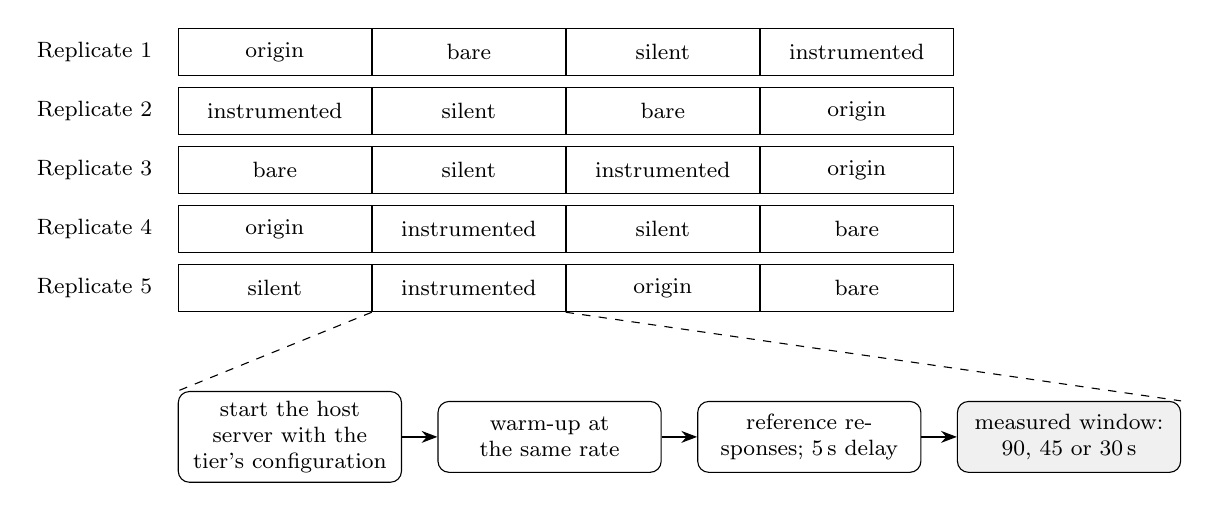
\begin{tikzpicture}[
    tier/.style={draw, minimum width=2.45cm, minimum height=6mm, font=\footnotesize, inner sep=1pt},
    lbl/.style={font=\footnotesize, anchor=east},
    cellstep/.style={draw, rounded corners, align=center, font=\footnotesize, minimum height=9mm},
    flow/.style={-{Stealth[length=2mm]}, thick}]
  \foreach \row/\a/\b/\c/\d in {1/origin/bare/silent/instrumented,
                                2/instrumented/silent/bare/origin,
                                3/bare/silent/instrumented/origin,
                                4/origin/instrumented/silent/bare,
                                5/silent/instrumented/origin/bare} {
    \node[lbl] at (0,-0.75*\row) {Replicate \row};
    \node[tier, anchor=west] (a\row) at (0.2,-0.75*\row) {\a};
    \node[tier, right=0pt of a\row] (b\row) {\b};
    \node[tier, right=0pt of b\row] (c\row) {\c};
    \node[tier, right=0pt of c\row] (d\row) {\d};
  }
  \node[cellstep, below=1.0cm of a5.south west, anchor=north west, text width=2.6cm] (s1)
    {start the host server with the tier's configuration};
  \node[cellstep, right=0.45cm of s1, text width=2.6cm] (s2) {warm-up at the same rate};
  \node[cellstep, right=0.45cm of s2, text width=2.6cm] (s3) {reference responses; 5\,s delay};
  \node[cellstep, right=0.45cm of s3, text width=2.6cm, fill=gray!12] (s4) {measured window:
    90, 45 or 30\,s};
  \draw[flow] (s1) -- (s2);
  \draw[flow] (s2) -- (s3);
  \draw[flow] (s3) -- (s4);
  \draw[dashed] (b5.south west) -- (s1.north west);
  \draw[dashed] (b5.south east) -- (s4.north east);
\end{tikzpicture}
\caption{One run of a variant at one rate: five replicates of the four tiers in a changing order (top) and the steps of one cell (bottom).}
\label{fig:method.run}
\end{figure}

A cost is computed within each replicate, as the difference between two of its cells, and then
summarised across the five replicates. The reported value is the median of the five differences,
and its uncertainty is given as their range, from the smallest to the largest. With five values, the
range is the nonparametric confidence interval of the median at a confidence level of 93.75\,\%,
the probability that the median of the distribution lies between the smallest and the largest of
five independent samples. Such intervals assume no particular distribution, which suits latency
measurements, whose distributions are skewed \cite{hoefler2015scientific}. A difference counts as
\emph{resolved} if all five differences have the same sign; if the range includes zero, the
measurement cannot tell the direction of the effect, and the result is reported as unresolved
rather than by its median.

Latency is reported \emph{per} \texttt{GET} request: within each cell, the mean of the median latencies of
the four \texttt{GET} probes, and from these the difference per replicate. The 95th percentile per
\texttt{GET} is formed in the same way.

\paragraph{In the in-server deployment.} The in-server variants are measured in the same four
tiers, but their origin tier is not evaluated. Their bare tier is the web server serving its own
pages without HDM, so silent minus bare keeps its meaning, the cost of HDM, and instrumented minus
silent the cost of the timing lines. The origin tier is not reported for them, for two reasons. First,
the origin tier serves RQ1.2, which asks what a reverse proxy adds between the client and the
server; in the in-server deployment, no proxy stands in between, so there is nothing for it to
measure. Second, compared with the origin tier, the bare tier would measure only the difference
between two web servers serving the same pages, OpenResty or Apache httpd against nginx, which
differ in version, build and configuration. That difference says nothing about HDM or about where
it runs, and it is not a question of this thesis. During their other tiers, nginx keeps running but receives no
requests; its CPU time per request should then be close to zero, which confirms that nothing was
forwarded.

\paragraph{Comparing variants.} Each variant is measured in a run of its own: the two Envoy
variants in one series of runs, the two in-server variants in another, days later. Within each run, every difference is paired. Between the runs,
nothing is, so variants are never compared by subtracting latencies measured in different runs,
which would let the drift between the runs decide the result. They are compared through
their paired differences: a variant is called cheaper than another only if the ranges of the two
differences do not overlap, following Hoefler and Belli's rule to compare nondeterministic data
through non-overlapping confidence intervals \cite{hoefler2015scientific}. If the ranges overlap,
this method cannot order the two variants.

%----------------------------------------------------------------------
\section{Measurement Planes}
\label{sec:method.planes}

Each cell is measured on three \emph{planes}, because no single one is reliable on its own on a
virtualised host (Table~\ref{tab:method.planes}).

\begin{table}[htbp]
\centering
\small
\begin{tabularx}{\textwidth}{@{}>{\raggedright\arraybackslash}p{2.6cm}>{\raggedright\arraybackslash}p{3.8cm}>{\raggedright\arraybackslash}X@{}}
\toprule
Plane & Source & Robust to, and used for \\
\midrule
End-to-end latency & k6, per probe, in milliseconds & what a client experiences; robust to drift
  only through pairing \\
CPU time per request & the control group of each container & the work a component performs; not
  affected by queueing, so it stays measurable where latency differences are lost \\
Timers inside HDM & the log of the host server, in microseconds, instrumented tier only & the cost of
  single operations per honeytoken type; affected by everything that delays the worker \\
\bottomrule
\end{tabularx}
\caption{The three measurement planes.}
\label{tab:method.planes}
\end{table}

\paragraph{Latency.} k6 records the duration of every probe, and for each probe and cell the
median and the percentiles from the 5th to the 99th are kept. Before the load starts, k6 sends every probe once
to the host server and once to the origin server and keeps both responses as references
(Figure~\ref{fig:method.run}). Every response during the measurement is compared with the host
server's reference by status and by a hash of the body; the share of identical responses is the
integrity metric of RQ3.2 (responses intact under load). k6 also records for every probe the share of requests that had to open a
new connection.

\paragraph{CPU time.} A sampler on the host reads the file \texttt{cpu.stat} of each container's
control group (\secrefp{sec:bg.perf}) four times per second. k6 marks the moment at which the
first measured iteration starts, and the CPU time is integrated over exactly the measured window from
that moment. It is divided by the number of requests the measured iterations sent, which gives the
CPU time per request, split into user and system time. Two properties of this figure matter for its
interpretation. First, it is an average over all nine requests of an iteration. With HDM, the SQL-injection trap
answers the four \texttt{POST} requests itself, or, in the WebAssembly variant, replaces the origin
server's answer (\secrefp{sec:impl.wasm}). Without HDM, the Envoy variants forward these
requests to the origin server and the in-server variants answer them with their own 404 page, so
the CPU time HDM adds is net of the work that the SQL-injection trap replaces. Second, VirtualBox does
not report the time during which the host takes a vCPU away from the guest; the guest's steal time
stayed zero. Such time is therefore billed to whatever process was running, and only pairing, not
the counter, protects against it.

A server also consumes CPU time when it is idle, and at one iteration per second this idle cost is
divided among few requests. The \emph{marginal} CPU time per request separates the two: for each
tier, the CPU time of all valid cells at all three rates is fitted as an idle cost per second times
the window's duration plus a marginal cost times the number of requests. A fit that requires a
negative idle or marginal cost is rejected as unphysical, and the CPU time per rate is reported
instead.

\paragraph{Timers inside HDM.} The timers of \secref{sec:impl.common} enclose the detection and
the insertion for each honeytoken type and the scan of the SQL-injection trap. All variants read a wall clock and
write whole microseconds, and most of the timed operations take one to five microseconds. A median
of such values can only be an integer, so the timers are summarised by a mean from which 5\,\% of the
samples have been trimmed at each end; the averaging recovers resolution below one microsecond, and
the trimming removes samples in which the worker was descheduled. The timers enclose only part of
what HDM does: entering and leaving the runtime, collecting the response body and writing the alert
lines lie outside them. The size of that part is itself a result (Chapter~\ref{chap:AB.results}).

\paragraph{Alerts.} From the host server's log, the alert lines and SQL-injection trap lines written during the measured
window are counted and compared with the seven alert lines and two SQL-injection trap lines that each iteration should
produce; on the bare tier, the count must be zero. Because alert lines are the only output of HDM's
detection, a detection that leaves no line counts as not made.

%----------------------------------------------------------------------
\section{Supplementary Experiments}
\label{sec:method.supp}

\paragraph{Functional matrix.} To answer RQ3.1 (the same response with and without HDM), each variant receives, without load, 13
requests whose responses the main workload does not contain: an HTML page, a page compressed with
gzip, a \texttt{HEAD} request, a conditional request, a range request for the first 100 bytes, an
empty response with status 204, a 404 page, a JSON (JavaScript Object Notation) document, a binary file, an HTML page without
\texttt{</body>}, HTML pages of 768\,KiB and 2\,MiB, and a request in HTTP/1.0. Each response of the
instrumented tier is compared with the same variant's response without HDM and classified as
\emph{preserved} (identical), \emph{injected} (HTML that differs only by inserted text, the intended
effect), \emph{changed} (a difference that the client can still use, such as a decoy header on a
JSON response), \emph{broken} (a response that the server without HDM would not have produced and that
the client cannot use, such as a different status, an undecodable body or deleted content) or \emph{not exercised}
(the server without HDM already refuses the request).

\paragraph{Request types and page size.} For RQ2.2 (where the added cost arises and how it grows with the size of a page), two further runs of the paired harness use other
workloads at fixed rates, in the bare, silent and instrumented tiers, with three replicates each.
The first sends only the unrecorded first request and the four \texttt{GET} probes, at 100
iterations per second; its difference from the main workload isolates what the four \texttt{POST}
requests to the SQL-injection trap cost, which the mixed CPU figure nets out. The second sends one \texttt{GET}
request each for pages of 1, 16, 256 and 768\,KiB, at 10 iterations per second, all below Envoy's
buffer limit (\secrefp{sec:bg.platforms}). In both, the host server's idle CPU time, measured
during the delay before the first iteration, is subtracted.

The request-type and page-size runs have no origin tier; each is paired within itself, which is all its
question requires.


%----------------------------------------------------------------------
\section{Run Validity}
\label{sec:AB.validity}

Every cell is assessed before it may enter a result. A cell that fails is kept in the result file
with the reasons for its rejection and excluded from every statistic. A cell is rejected if any of
the following holds:
\begin{itemize}
  \item k6 placed less than 95\,\% of the offered iterations, or dropped more than 1\,\% of them;
  \item more than 0.5\,\% of the requests failed;
  \item more than 1\,\% of the timer samples of an operation, and at least three samples, exceeded
    one millisecond, a duration that no timed operation of the main workload needs and that
    indicates that the host took the processor away; this gate can be applied only to the
    instrumented tier. In the page-size runs, inserting honeytokens into the largest page takes
    about a millisecond in Apache in-server, so the gate also rejects its instrumented cells there;
    these runs are evaluated on the bare and silent tiers, which the gate does not read;
  \item the origin server used more than 1,000\us{} of CPU time per request. The origin server is
    the same in every cell and is not under test, so a high value can only mean that the host was
    disturbed. The threshold lies about three times above the highest value observed in undisturbed
    cells, and it does not refer to the quantity being measured, so it cannot favour a result;
  \item the guest's kernel log reports, inside the measured window, a soft lockup or a jump of the
    clock, which shows that the host stopped running the VM.
\end{itemize}
A crash of a worker process is recorded as a warning but does not reject a cell by itself. A
crashing worker takes the request in flight with it, and that damage is measured directly by the
gates on failed requests and placed iterations. The worker processes of Apache in-server crashed
several times in every run with HDM at 100 iterations per second, while those cells passed every
other gate. Rejecting every cell with a crash would have discarded these load levels, and with them
exactly the measurements in which the crashes are the finding. All cells are judged by the same rules.

All 240 cells of the paired benchmark were valid: 60 for each variant, five replicates of four tiers
at three rates.

%----------------------------------------------------------------------
\section{What the Method Cannot Resolve}
\label{sec:method.limits}

The measures above leave limits that the results must respect.

\begin{itemize}
  \item \emph{Absolute values.} All values come from one virtualised host, so they hold for this
    testbed only; the comparisons between the variants are the claims the results support.
  \item \emph{Small differences.} Even paired and replicated, the end-to-end latency resolves
    differences of tens of microseconds at best. A cost that small would be reported as
    unresolved, and no conclusion would be drawn from it.
  \item \emph{The host.} VirtualBox gives the guest no control over which physical core runs a vCPU,
    and the processor has cores of two different speeds, so a vCPU can move between them during a
    measurement. Steal time is not reported (\secrefp{sec:method.planes}). Pairing distributes
    such disturbances over the tiers but does not remove them.
  \item \emph{The tail.} Latency far above the median is dominated by the host. The gates remove
    cells in which this dominates; they do not explain the tail that remains.
  \item \emph{Image versions.} The container images are referenced by tags that can move, and
    their identifiers were recorded for the run of the in-server variants only, so it cannot be shown
    that both runs used the same images of the load generator and the origin server.
  \item \emph{Comparisons across runs.} Variants measured in different runs are compared only
    through their paired differences, and overlapping ranges leave them unordered
    (\secrefp{sec:method.tiers}).
\end{itemize}

Chapter~\ref{chap:discussion} returns to these limits when it assesses the threats to the validity of
the results. Chapter~\ref{chap:AB.results} now presents the results, one research question at a
time.

%======================================================================
\chapter{Results}
\label{chap:AB.results}

This chapter presents the measurements of the four variants, one research question at a time. All
240 cells of the paired benchmark were valid (\secrefp{sec:AB.validity}), so every result below
rests on five paired replicates per variant, tier and load level. Each value is the median of the
five paired differences, and the whiskers in the figures show their range, from the smallest to
the largest (\secrefp{sec:method.tiers}). The two Envoy variants and the two in-server variants
were measured in separate runs, so a statement that one variant costs more than another is made
only where the two ranges do not overlap. The variants appear in the same order and with the same
colours and markers in every figure: the two proxy variants, Envoy Lua and Envoy WebAssembly,
first, and the two in-server variants, OpenResty in-server and Apache in-server, second; bars of
the in-server variants are hatched.

%----------------------------------------------------------------------
\section{RQ1: Latency Added}
\label{sec:results.rq1}

\subsection{Latency Added by HDM}

Figure~\ref{fig:results.latency} shows how much HDM adds to the latency of a \texttt{GET} request,
the difference between the silent tier and the bare tier, averaged over the four \texttt{GET}
probes, at the three load levels. At the median
(left), OpenResty in-server adds the least, 69 to 81\us, followed by Envoy WebAssembly with 110
to 150\us{} and Envoy Lua with 147 to 203\us; Apache in-server adds the most, 183 to 244\us.
Relative to the latency of the same host server without HDM, this is 13 to 20\,\% for OpenResty
in-server, 12 to 18\,\% for Envoy WebAssembly, 18 to 22\,\% for Envoy Lua and 32 to 48\,\% for
Apache in-server. All 60 differences are resolved: in every variant, at every load level, all five
replicates agree that HDM makes a \texttt{GET} request slower.

The ranges separate OpenResty in-server from every other variant at every load level. Between Envoy
Lua and Envoy WebAssembly, the medians favour the WebAssembly variant at every load level, but the
ranges overlap or touch, so the two cannot be ordered. Apache in-server adds more than Envoy Lua
only at 100 iterations per second, where the ranges no longer overlap. Apache in-server also
inserts honeytokens into fewer responses per iteration than the other variants, three of the five
HTML responses instead of five (\secrefp{sec:impl.apache}); its cost therefore covers less
insertion work.

\begin{figure}[tbp]
\centering
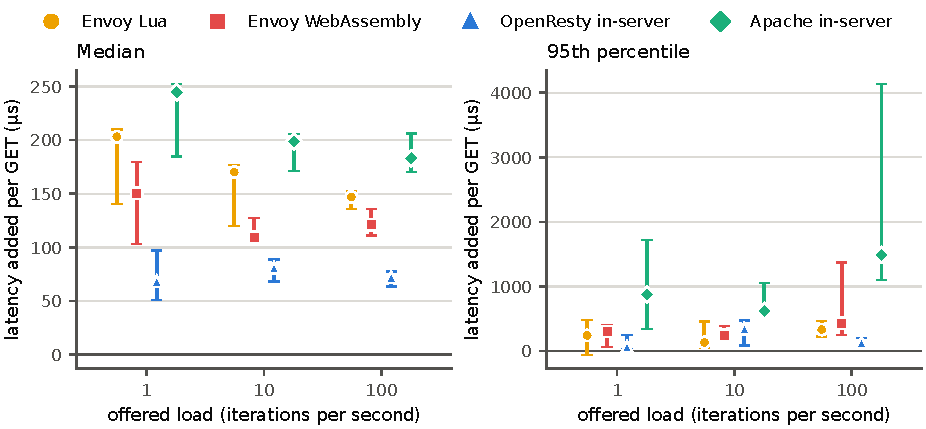
\includegraphics[width=\textwidth]{latency_added.pdf}
\caption{Latency that HDM adds to a \texttt{GET} request at the median (left) and at the 95th percentile (right), for the three load levels.}
\label{fig:results.latency}
\end{figure}

With increasing load, the latency HDM adds stays at the same order of magnitude in every variant.
In the two Envoy variants and in Apache in-server, the median is lower at 100 iterations per second
than at 1, by 29 to 61\us; in OpenResty in-server, the three medians lie within 12\us{} of each
other. Because the host servers without HDM themselves answer faster at 100 iterations per second
(for the Envoy variants, Figure~\ref{fig:results.levels}), the relative cost is higher there than at 10 iterations per
second in every variant.

The 95th percentile (right of Figure~\ref{fig:results.latency}) shows how HDM affects the slowest
requests. In the two Envoy variants and in OpenResty in-server, HDM adds between 71 and 435\us{} at
this percentile, and in all variants except Envoy Lua at 10 iterations per second, the addition is
larger at the 95th percentile than at the median: HDM stretches the slow end of the distribution
more than its middle. Apache in-server stands out: it adds 880, 622 and 1,491\us{} at the three
load levels, with ranges reaching 4,132\us{} at 100 iterations per second. Envoy Lua's range at 1
iteration per second includes zero; at that load, its effect on the slowest requests cannot be
distinguished from the noise of the testbed.

\subsection{Latency of the Reverse Proxy}
\label{sec:results.hostlatency}

In the proxy deployment, HDM is only part of what the deployment adds.
Figure~\ref{fig:results.levels} shows the absolute median latency of a \texttt{GET} request for the
two Envoy variants in three configurations: sent directly to the origin server, through Envoy
without HDM, and through Envoy with HDM. The distance from the hollow to the filled marker is what
HDM adds; the distance from the grey circle to the hollow marker is what the reverse proxy adds
without HDM.

\begin{figure}[tbp]
\centering
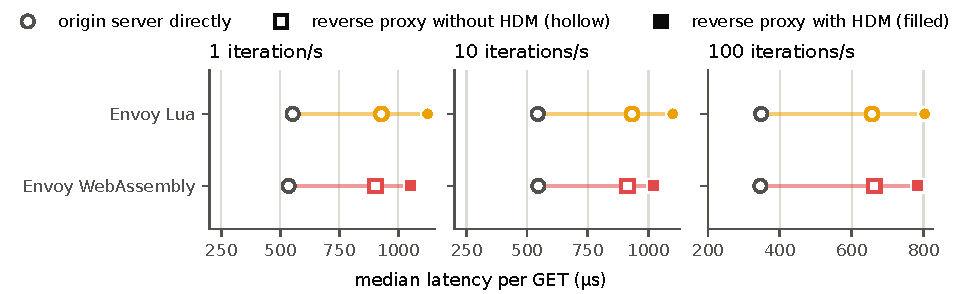
\includegraphics[width=\textwidth]{latency_levels.pdf}
\caption{Median latency of a \texttt{GET} request in the Envoy variants, sent directly to the origin server (grey circle), to Envoy without HDM (hollow marker) and to Envoy with HDM (filled marker).}
\label{fig:results.levels}
\end{figure}

The reverse proxy alone adds more than HDM does. Without HDM, Envoy adds
396, 389 and 309\us{} per \texttt{GET} request over direct access to the origin server in the Lua
variant and 372, 369 and 319\us{} in the WebAssembly variant, at 1, 10 and 100 iterations per
second; this includes the additional pass over the network between the containers
(\secrefp{sec:method.tiers}). Of what the deployed stack adds above the origin server, HDM
accounts for 30 to 34\,\% in Envoy Lua and for 23 to 29\,\% in Envoy WebAssembly. With HDM, a
\texttt{GET} request through Envoy takes 442 to 571\us{} longer than one sent directly to the origin
server. Measured against the origin tier instead of the bare tier, HDM's cost in the Envoy variants
would therefore appear about three to four times as large, which is why every cost of HDM in this chapter
is taken against the bare tier (\secrefp{sec:method.tiers}).

\subsection{Reconnections}

In Apache in-server, HDM changes how the client's connections are used. Apache httpd closes the
connection after each response of the SQL-injection trap with status 500, so the request that
follows must open a new one (\secrefp{sec:method.workload}). With HDM, 12 to 25\,\% of each
probe's requests opened a new connection at every load level, against at most 0.9\,\% without HDM.
The other three variants kept their connections open.

\subsection{Answer to RQ1}

HDM adds 69 to 81\us{} to the median latency of a \texttt{GET} request in OpenResty in-server, 110 to
150\us{} in Envoy WebAssembly, 147 to 203\us{} in Envoy Lua and 183 to 244\us{} in Apache in-server,
12 to 48\,\% of the latency without HDM (RQ1.1). At the 95th percentile, the addition is larger,
and in Apache in-server it reaches several milliseconds at the highest load. In the proxy
deployment, the reverse proxy itself adds 309 to 396\us, more than HDM does (RQ1.2). With increasing load, the
absolute cost of HDM stays at the same level or falls slightly, while its share of the total
latency grows (RQ1.3).

%----------------------------------------------------------------------
\section{RQ2: CPU Time}
\label{sec:results.rq2}

\subsection{CPU Time per Request}

Latency includes time spent waiting; CPU time measures only the work done
(\secrefp{sec:method.planes}). Figure~\ref{fig:results.cpu} shows the CPU time HDM adds per
request, the difference between the silent tier and the bare tier, averaged over all nine requests
of an iteration. At 1 iteration per second, the ranges are wide, because the host servers' idle CPU
time is divided among few requests; at 10 and 100 iterations per second, they narrow. The marginal
CPU time per request (right), fitted over all three load levels, removes the idle cost: HDM costs 32
(25 to 36)\us{} per request in OpenResty in-server, 45 (39 to 50)\us{} in Envoy Lua, 108 (99 to
121)\us{} in Envoy WebAssembly and 261 (229 to 334)\us{} in Apache in-server. The ranges of the four
variants do not overlap: in CPU time, the order is clear.

\begin{figure}[tbp]
\centering
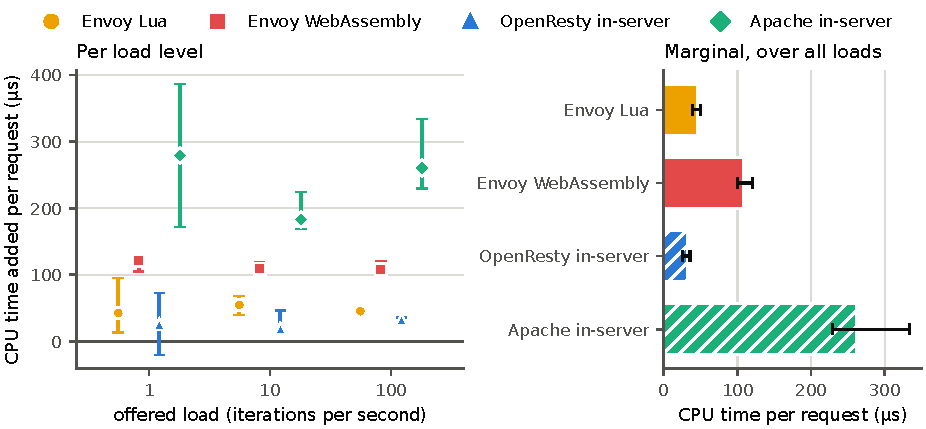
\includegraphics[width=\textwidth]{cpu_added.pdf}
\caption{CPU time that HDM adds per request, per load level (left) and as the marginal time fitted over all three load levels (right).}
\label{fig:results.cpu}
\end{figure}

The order in CPU time differs from the order in latency. Envoy WebAssembly adds less latency than
Envoy Lua at the median, but more than twice its CPU time. The host server's CPU time does not wait
for the network, and a request's latency includes waiting; the two measures therefore need not
rank the variants alike.

\subsection{Where the Cost Arises}
\label{sec:results.where}

The timers inside HDM measure only its detection and insertion operations
(\secrefp{sec:method.planes}). Figure~\ref{fig:results.scopes} sets their total against the CPU
time and the latency that HDM adds, all per iteration at 100 iterations per second. The timed
operations take 54\us{} per iteration in Envoy WebAssembly and OpenResty in-server, 79\us{} in Envoy
Lua and 110\us{} in Apache in-server. The CPU time that HDM adds is several times larger: 286\us{} in
OpenResty in-server, 409\us{} in Envoy Lua, 973\us{} in Envoy WebAssembly and 2,353\us{} in Apache
in-server. Across the three load levels, the timed operations account for 17 to 22\,\% of the added
CPU time in Envoy Lua and 19 to 35\,\% in OpenResty in-server, but only 5 to 7\,\% in Envoy
WebAssembly and in Apache in-server. Most of what HDM costs therefore lies outside its detection and
insertion code, in work that no timer encloses, such as entering and leaving the runtime, collecting
the response body and writing alert lines (\secrefp{sec:method.planes}). This part is largest in
Envoy WebAssembly, whose module reaches every request and response only through calls into Envoy
(\secrefp{sec:impl.wasm}), and in Apache in-server, whose code is interpreted.

\begin{figure}[tbp]
\centering
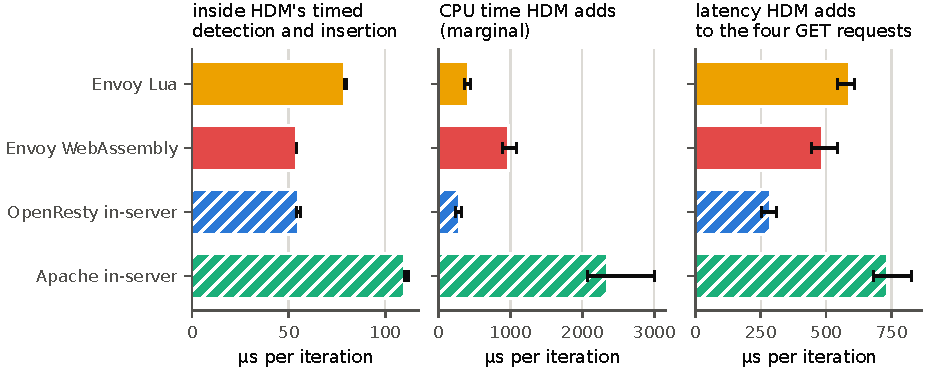
\includegraphics[width=\textwidth]{cost_scopes.pdf}
\caption{Three measures of HDM's cost per iteration at 100 iterations per second, each on its own scale: the time inside HDM's timed operations (left), the added CPU time as a marginal fit (middle) and the latency added to the four \texttt{GET} requests (right).}
\label{fig:results.scopes}
\end{figure}

The timing lines of the instrumented tier have a cost of their own. The marginal CPU time of the
instrumented tier exceeds that of the silent tier by 21\us{} per request in OpenResty in-server,
41\us{} in Envoy Lua, 64\us{} in Envoy WebAssembly and 144\us{} in Apache in-server, in the first two
variants a cost close to that of HDM itself. This is why the silent tier, not the instrumented one,
is the basis of every cost reported in this chapter (\secrefp{sec:method.tiers}).

\subsection{GET Requests and the SQL-Injection Trap}

The CPU figures above average over all nine requests of an iteration, four of which go to the
SQL-injection trap. The request-type runs separate the two (\secrefp{sec:method.supp});
Table~\ref{tab:results.mechanisms} shows the result at 100 iterations per second.

\begin{table}[tbp]
\centering
\small
\begin{tabularx}{\textwidth}{@{}X>{\raggedleft\arraybackslash}p{4.0cm}>{\raggedleft\arraybackslash}p{4.4cm}@{}}
\toprule
Variant & per \texttt{GET} request (\textmu s) & per request to the SQL-injection trap (\textmu s) \\
\midrule
Envoy Lua & $+165$ ($+66$ to $+175$) & $-109$ ($-118$ to $+16$) \\
Envoy WebAssembly & $+162$ ($+128$ to $+387$) & $+50$ ($-213$ to $+82$) \\
OpenResty in-server & $+77$ ($+66$ to $+101$) & $-28$ ($-48$ to $-3$) \\
Apache in-server & $+238$ ($+213$ to $+247$) & $+276$ ($+254$ to $+455$) \\
\bottomrule
\end{tabularx}
\caption{CPU time that HDM adds per \texttt{GET} request and per request to the SQL-injection trap, at 100 iterations per second.}
\label{tab:results.mechanisms}
\end{table}

On a \texttt{GET} request, HDM costs 77\us{} of CPU time in OpenResty in-server, 162 and 165\us{} in
the two Envoy variants and 238\us{} in Apache in-server. A request to the SQL-injection trap costs
less with HDM than without it in OpenResty in-server: without HDM, OpenResty answers these requests
with its own 404 page; with HDM, the SQL-injection trap answers them. In Envoy Lua,
the trap answers without forwarding the request to the origin server, and the range of its
difference includes zero. In Envoy WebAssembly, whose trap still forwards the request
(\secrefp{sec:impl.wasm}), the range includes zero as well. Only in Apache in-server does the
trap clearly cost CPU time, 276\us{} per request.

\subsection{Page Size}

The benchmark's pages are small, between 864 and 1,396 bytes. Figure~\ref{fig:results.size} shows
what HDM adds to the latency of a request for pages of 1, 16, 256 and 768\,KiB, as the median and
range of three paired replicates, two for Apache in-server. For pages up to
16\,KiB, the addition stays below 210\us{} in every variant. From 256\,KiB on, it grows roughly in
proportion to the size of the page, as expected of a module that collects the whole body and
searches it for the places to insert (\secrefp{sec:design.pipeline}): for a page of 768\,KiB, HDM adds 889\us{} in Envoy
WebAssembly, 1,372\us{} in Envoy Lua, 1,628\us{} in OpenResty in-server and 2,167\us{} in Apache
in-server. In OpenResty in-server, the 16\,KiB page costs more than the 1\,KiB page by a margin that
all three replicates confirm (199 to 252\us{} against 43 to 58\us); these measurements do not show
why. For Apache in-server, two of the three replicates are valid (\secrefp{sec:AB.validity}).

\begin{figure}[tbp]
\centering
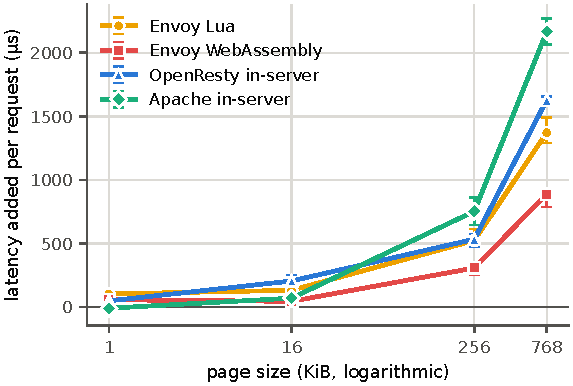
\includegraphics[width=0.62\textwidth]{page_size.pdf}
\caption{Latency that HDM adds to a request against the size of the page at 10 iterations per second, on a logarithmic horizontal axis.}
\label{fig:results.size}
\end{figure}

\subsection{Answer to RQ2}

HDM adds a marginal CPU time of 32\us{} per request in OpenResty in-server, 45\us{} in Envoy Lua,
108\us{} in Envoy WebAssembly and 261\us{} in Apache in-server; the ranges do not overlap (RQ2.1).
Only 5 to 35\,\% of that time is spent inside HDM's detection and insertion operations; the rest is
spent around them, most of all in Envoy WebAssembly and Apache in-server. Per request, HDM costs
more on a \texttt{GET} request than on a request to the SQL-injection trap, which in three variants
costs no more CPU time than the response it replaces. The cost grows roughly in proportion to the
size of the page from 256\,KiB on (RQ2.2).

%----------------------------------------------------------------------
\section{RQ3: Functional Correctness}
\label{sec:results.rq3}

\subsection{Other Kinds of Response}

Table~\ref{tab:results.matrix} shows how each variant treats the response types of the functional
matrix (\secrefp{sec:method.supp}), each compared with the same variant's response without HDM.

\begin{table}[tbp]
\centering
\small
\begin{tabularx}{\textwidth}{@{}X*{4}{>{\centering\arraybackslash}p{2.2cm}}@{}}
\toprule
Response & Envoy Lua & Envoy WebAssembly & OpenResty in-server & Apache in-server \\
\midrule
HTML page & injected & injected & injected & injected \\
HTML page, compressed with gzip & \textbf{broken} & \textbf{broken} & injected & injected \\
\texttt{HEAD} request & \textbf{broken} & changed & changed & preserved \\
Conditional request & changed & changed & changed & changed \\
Range request (first 100 bytes) & \textbf{broken} & \textbf{broken} & \textbf{broken} & preserved \\
Empty response (204) & changed & changed & changed & preserved \\
Page not found (404) & injected & injected & injected & preserved \\
JSON document & changed & changed & changed & changed \\
Binary file & changed & changed & changed & changed \\
HTML without \texttt{</body>} & injected & injected & injected & injected \\
HTML page of 768\,KiB & injected & injected & injected & injected \\
HTML page of 2\,MiB & \textbf{broken} & \textbf{broken} & injected & injected \\
HTTP/1.0 request & not exercised & not exercised & injected & injected \\
\bottomrule
\end{tabularx}
\caption{The response of each variant with HDM, compared with its response without HDM
(\secrefp{sec:method.supp} defines the categories).}
\label{tab:results.matrix}
\end{table}

Three kinds of response break in the proxy deployment. Both Envoy variants insert honeytokens into
the compressed bytes of a gzip-encoded page, which the client can then no longer decode; they
modify the partial content of a range request, which corrupts the resource the client reassembles;
and they fail to deliver a page of 2\,MiB, which exceeds Envoy's buffer limit
(\secrefp{sec:bg.platforms}). Envoy Lua also answers a \texttt{HEAD} request with the length of
the page without honeytokens, while the corresponding \texttt{GET} returns the longer page.

The in-server variants avoid most of these failures. Both deliver the compressed page with its
honeytokens and in a form the client can decode, and both deliver the 2\,MiB page. Apache
in-server answers the range request with a correct part of the page with honeytokens and the
\texttt{HEAD} request with the length of that page. OpenResty in-server answers the range request
with the whole page with honeytokens and status 200: HTTP allows a server to ignore a range request
in this way \cite{rfc9110}, but the client receives more than it asked for, and the matrix counts
the change of status as broken. In Apache in-server, the 204 response and the 404 page are
preserved because HDM does not act on them (Sections~\ref{sec:impl.apache}, \emph{\nameref{sec:impl.apache}}, and~\ref{sec:AB.level}, \emph{\nameref{sec:AB.level}}).
The responses classified as changed carry the decoy header on a response that is not HTML, lack the
\texttt{Content-Length} header of a \texttt{HEAD} response, or are sent in pieces instead of with a
stated length; none of these prevents the client from using them.

\subsection{Integrity under Load and Detection}

Under load, every measured response was compared with the reference response the same tier returned
before the load started (\secrefp{sec:method.planes}). Envoy Lua, Envoy WebAssembly and
OpenResty in-server returned every response intact at every load level, and they wrote every
expected alert line and SQL-injection trap line. Apache in-server returned 99.78\,\% of its
responses intact at 10 and 99.77\,\% at 100 iterations per second in the silent tier, and it wrote
99.98\,\% of the expected alert lines and 99.95\,\% of the expected SQL-injection trap lines at 100 iterations per
second, consistent with the crashes of its worker processes (\secrefp{sec:results.rq4}).
No variant wrote an alert line without HDM.

\subsection{Answer to RQ3}

Apart from the honeytokens, HDM changes responses in every variant, but it breaks them mainly in the
proxy deployment: compressed pages, range requests and pages above Envoy's buffer limit fail in both
Envoy variants, and Envoy Lua also misreports the length of a \texttt{HEAD} response. In the
in-server deployment, only OpenResty's answer to a range request changes its status (RQ3.1). Under
load, three variants keep every response intact and Apache in-server keeps 99.77\,\% or more
(RQ3.2). Every variant raises every expected alert except Apache in-server, which misses at most
0.05\,\% of them as deployed, and no variant raises an alert without HDM (RQ3.3).

%----------------------------------------------------------------------
\section{RQ4: Influence of the Runtime and the Deployment}
\label{sec:results.rq4}

\subsection{HDM's Operations per Honeytoken Type}

Figure~\ref{fig:results.timers} shows how long HDM's detection and insertion take for each
honeytoken type, measured by the timers of the instrumented tier at 10 iterations per second. Every
operation takes between 0.35 and 5.3\us. Apache in-server, the only variant whose code is
interpreted by PUC Lua, needs the most time for every detection, 1.7 to 5.3\us, and for the three
insertions into the body, 2.7 to 4.5\us. The two Envoy variants, which share a host server and
differ only in the runtime, lie within 1.4\us{} of each other in every operation: LuaJIT is faster
in detecting HTML comments, HTTP headers and decoy paths, WebAssembly in detecting cookies and form
fields and in every insertion. Setting a decoy header or a cookie takes longer in the two Envoy variants, 1.6 to
3.3\us, than in the two web servers, 0.35 to 1.5\us. At 1 and 100 iterations per second, the values
are similar; most are somewhat higher at 1 iteration per second.

\begin{figure}[tbp]
\centering
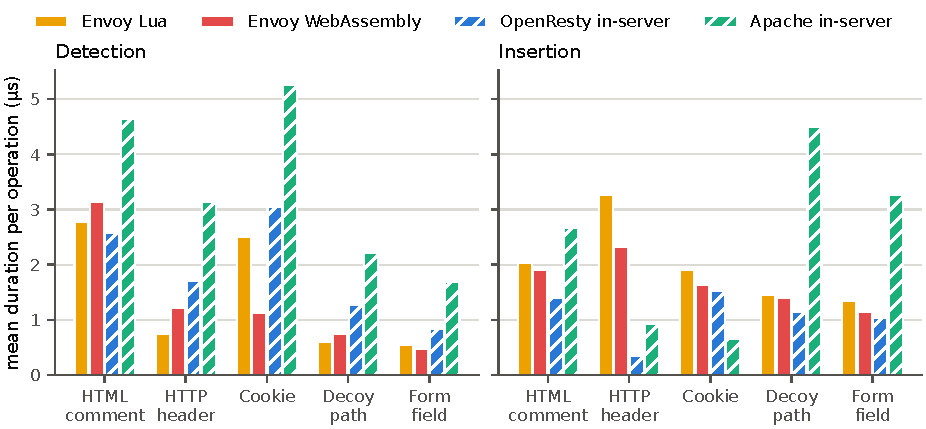
\includegraphics[width=\textwidth]{hdm_timers.pdf}
\caption{Mean duration of HDM's detection (left) and insertion (right) per honeytoken type at 10 iterations per second.}
\label{fig:results.timers}
\end{figure}

These durations are small compared with what HDM adds in total. Envoy WebAssembly needs about as
much time for its operations as OpenResty in-server (Figure~\ref{fig:results.scopes}), yet it adds
more than three times the CPU time per request (Figure~\ref{fig:results.cpu}). The runtime therefore
matters less through the speed of the detection and insertion code itself than through the work
around it.

\subsection{The SQL-Injection Trap: Decoding and Scanning}

The four probes of the SQL-injection trap form a two-by-two design (\secrefp{sec:method.workload}).
Within each replicate, the difference between the encoded and the plain probes is the cost of
decoding the input, and the difference between the clean logins and the signature hits is the cost
of scanning further through the list of signatures. Table~\ref{tab:results.sqli} shows both at 100
iterations per second.

\begin{table}[tbp]
\centering
\small
\begin{tabularx}{\textwidth}{@{}X>{\raggedleft\arraybackslash}p{3.0cm}>{\raggedleft\arraybackslash}p{3.0cm}>{\raggedleft\arraybackslash}p{3.0cm}@{}}
\toprule
Variant & signature hit, plain (\textmu s) & decoding (\textmu s) & scanning further (\textmu s) \\
\midrule
Envoy Lua & 7.4 & 1.26 (1.22 to 1.30) & 0.73 (0.67 to 0.78) \\
Envoy WebAssembly & 2.7 & 0.09 (0.08 to 0.10) & 0.51 (0.50 to 0.53) \\
OpenResty in-server & 6.9 & 1.42 (1.36 to 1.56) & 0.82 (0.70 to 0.86) \\
Apache in-server & 16.0 & 1.43 (1.32 to 1.48) & 2.84 (2.51 to 2.88) \\
\bottomrule
\end{tabularx}
\caption{Duration of the SQL-injection trap's work at 100 iterations per second.}
\label{tab:results.sqli}
\end{table}

The trap's work takes 2.7\us{} in Envoy WebAssembly, about 7\us{} in the two LuaJIT variants and
16\us{} in Apache in-server. Decoding costs 1.3 to 1.4\us{} in all three Lua variants, whether LuaJIT
or PUC Lua runs them, and almost nothing in WebAssembly. Scanning further costs 0.5 to 0.8\us{} in
LuaJIT and WebAssembly and 2.8\us{} in PUC Lua, the only runtime in which the length of the list of
signatures matters noticeably.

\subsection{Stability of Apache httpd}

The worker processes of Apache in-server crashed with HDM. At 100 iterations per second, they
crashed 10 to 12 times in every run of the silent tier and 9 to 12 times in every run of the
instrumented tier; at 10 iterations per second, they crashed two or three times in three runs. They
never crashed without HDM, and no other variant crashed. Each crash takes the request in flight with
it (\secrefp{sec:AB.validity}). Apache in-server keeps one Lua state per thread
(\secrefp{sec:impl.apache}); whether another lifetime of the state avoids the crashes was not
measured for this variant.

\subsection{Reverse Proxy and Web Server on the Same Runtime}

Envoy Lua and OpenResty in-server both run HDM on LuaJIT, the first in a reverse proxy and the
second in the web server that serves the pages (RQ4.3). Their detections take similar time: in
Figure~\ref{fig:results.timers}, the two lie within 1\us{} of each other in every detection, and
their trap scans take about 7\us{} in both (Table~\ref{tab:results.sqli}). Their total cost
differs. OpenResty in-server adds 69 to 81\us{} to the median latency of a \texttt{GET} request,
Envoy Lua 147 to 203\us, with ranges that do not overlap at any load level. In CPU time, their ranges
overlap at 1 and 10 iterations per second, and at 100 iterations per second, OpenResty in-server adds
less, 32 against 45\us. OpenResty in-server also delivers compressed pages and pages of 2\,MiB
correctly, which Envoy Lua does not (Table~\ref{tab:results.matrix}). Because the two variants differ
in the host server as well as in the deployment, these differences cannot be attributed to the
deployment alone.

\subsection{Answer to RQ4}

The runtime determines how long HDM's operations take, but these operations are a small part of its
cost. Each takes at most 5.3\us; PUC Lua is the slowest runtime, and LuaJIT and WebAssembly differ by
at most 1.4\us{} (RQ4.1). In the SQL-injection trap, decoding costs about 1.3\us{} in every Lua
runtime and almost nothing in WebAssembly, and scanning the whole list of signatures costs
noticeably more only in PUC Lua (RQ4.2). What separates the variants is the work around these
operations, which in Envoy WebAssembly and Apache in-server costs far more than the operations
themselves. With the runtime held fixed, the web
server adds less latency and delivers more kinds of response correctly than the reverse proxy,
although the difference in server prevents attributing this to the deployment alone (RQ4.3).

%======================================================================
\chapter{Discussion}
\label{chap:discussion}
What the results mean, and how far they can be trusted.

\section{Synthesis across Research Questions}
One table of the four variants against the four answers.

\section{Choosing a Deployment and a Variant}
A trade-off summary per variant: latency, CPU, robustness. Then the deployment: the in-server
deployment saves the extra hop and the extra server process, but it requires the application's
pages to be served by nginx or Apache httpd and changes that server's configuration; a reverse proxy
can be placed in front of any origin, including application servers that are not web servers of
this kind. Apache in-server inserts no honeytokens into its own error pages
(\secrefp{sec:impl.apache}).

\section{Where the Cost Comes From}
Runtime entry and exit, body buffering and log writes, not the detection logic.

\section{Deployment Implications}
Compressed bodies, range requests, preserved ETags, body-size limits.

\section{Threats to Validity}
A single VM host, synthetic traffic, moving image tags, timer resolution. Every variant was measured
in a run of its own, and the Envoy and in-server variants in different series days apart, so
variants are compared only through paired differences. Capacity is not compared, because the
in-server variants run on two cores against the Envoy variants' two plus the origin's one. Apache in-server does less insertion work per
iteration than the other variants. Envoy Lua and OpenResty in-server share a runtime but differ in
server as well as deployment (RQ4.3).

\section{Limitations}
POST-body inspection exists in only two of the four variants; no real attacker traffic; no TLS or
HTTP/2; no in-server variant for Envoy, which serves no files; the web servers were not studied as
reverse proxies.

%======================================================================
\chapter{Conclusion and Future Work}
\label{chap:conclusion}
\section{Summary}
RQ1--RQ4 answered in one or two sentences each, then the overall contribution.
\section{Future Work}
POST-body inspection in all variants, injecting into compressed bodies, a field study with real
attackers, TLS and HTTP/2. A capacity comparison with matched cores, honeytokens in Apache's own
error pages, and in-server variants of further web servers.

%======================================================================
\appendix
\chapter{Configuration Reference}
Every \texttt{config.json} field per honeytoken type, and the SQL-injection trap's fields. The
server configurations of the four variants with their configurations without HDM: Envoy Lua
(\texttt{envoy/envoy.yaml}), Envoy WebAssembly (\texttt{envoy-wasm/envoy-wasm.yaml}), OpenResty
in-server (\texttt{nginx/nginx-inserver.conf}) and Apache in-server (\texttt{httpd-inserver.conf}).
\material{\repo{CONTEXT.md}, \repo{docs/EDGE_LEVELING.md} (In-server deployment)}
\chapter{Parity-Check Request Set}
\label{app:parity}
The 13 requests and the documented exclusions, and the rules: status, decoy header and cookies on
every request, body hash only where the reference (OpenResty in-server) returned 200, identical
alert lines, no request at the origin server from the in-server variants, and identical forwarded
requests without trigger keywords from the Envoy variants.
\material{\repo{benchmarks/parity_check.py}, \repo{benchmarks/results/parity_check_2026-10-19.txt}}
\chapter{Reproducing the Benchmarks}
Commands, machine configuration, run durations: \texttt{run\_paired\_benchmark.py} for the Envoy
variants, \texttt{run\_inserver\_suite.sh} for the in-server variants, and the request-type and
page-size runs.
\material{\repo{docs/BENCHMARK_METHODOLOGY.md} \S3--4, \S10; \repo{benchmarks/README.md}}
\chapter{Additional Result Tables}
Per-rate tables and figures.
\material{\repo{benchmarks/results/plots/by_rate/}}

\bibliographystyle{ieeetr}
\bibliography{sources}
\end{document}
